% ===================================================================
%  Poros: QLoRA Fine-Tuning of Models Larger Than the GPU by Streaming the Frozen Base
%  Caistro Labs technical report.  Build: see ../Makefile (xelatex).
%
%  Numbers.  Every measured value in this file is a macro \nv{key}.  The
%  values are written to values.tex by launch_results.py from the logs;
%  a key the script could not fill prints a visible [pending] marker, and
%  `make final' refuses to build while any marker remains.  Do not type a
%  measured number into this file.
% ===================================================================
\documentclass[11pt,letterpaper]{article}

% -- Page --------------------------------------------------------------
\usepackage[letterpaper,textwidth=5.85in,textheight=8.75in,
            top=1.1in,headsep=0.3in,footskip=0.45in]{geometry}

% -- Fonts: Charter for text and math, Geist for display and figures ------
\usepackage{amsmath}
\usepackage{fontspec}
\usepackage{unicode-math}
\providecommand{\fontdir}{../fonts/}% the arXiv bundle sets ./
\setmainfont{XCharter}[
  Path           = \fontdir,
  Extension      = .otf,
  UprightFont    = *-Roman,
  BoldFont       = *-Bold,
  ItalicFont     = *-Italic,
  BoldItalicFont = *-BoldItalic,
  Numbers        = {Lining},
]
\setsansfont{Geist}[
  Path           = \fontdir,
  Extension      = .otf,
  UprightFont    = *-Regular,
  BoldFont       = *-SemiBold,
  ItalicFont     = *-Italic,
  BoldItalicFont = *-SemiBoldItalic,
  Scale          = MatchLowercase,
]
\setmonofont{GeistMono}[
  Path           = \fontdir,
  Extension      = .otf,
  UprightFont    = *-Regular,
  BoldFont       = *-Bold,
  Scale          = MatchLowercase,
]
\setmathfont{XCharter-Math.otf}[Path = \fontdir]
\newfontfamily\tabfigs{XCharter}[
  Path = \fontdir, Extension = .otf,
  UprightFont = *-Roman, BoldFont = *-Bold, ItalicFont = *-Italic,
  Numbers = {Lining,Monospaced}]
\linespread{1.06}

\usepackage[protrusion=true]{microtype}

% -- Colour: the Caistro landing-page tokens (app/globals.css, --color-lp-*) --
\usepackage{xcolor}
\definecolor{lpfg}{HTML}{18181B}       % --color-lp-foreground: text
\definecolor{lpnight}{HTML}{111111}    % --color-lp-night: headings
\definecolor{lpmuted}{HTML}{71717A}    % --color-lp-muted: secondary text
\definecolor{lpaccent}{HTML}{FF6B35}   % --color-lp-accent: Poros, and nothing else
\definecolor{lpaccentlt}{HTML}{FFE1D7} % --color-lp-accent-light: Poros tints
\definecolor{lppaper}{HTML}{FAFAF8}    % --color-lp-paper: panels
\definecolor{lprule}{HTML}{D4D4D8}     % hairlines (neutral grey)
\definecolor{lpbase}{HTML}{A1A1AA}     % baselines in figures (neutral grey)
\AtBeginDocument{\color{lpfg}}

% -- Structure ----------------------------------------------------------
\usepackage{graphicx}
\usepackage{booktabs}
\usepackage{array}
\usepackage{longtable}
\usepackage{colortbl}
\usepackage{multirow}
\usepackage{caption}
\usepackage{subcaption}
\usepackage{enumitem}
\usepackage{fancyhdr}
\usepackage[explicit]{titlesec}
\usepackage{needspace}
\usepackage{etoolbox}
\usepackage{tikz}
\usetikzlibrary{positioning,calc,arrows.meta,shapes.geometric,fit,backgrounds}
\usepackage{framed}
\newenvironment{claimbox}{%
  \def\FrameCommand{{\color{lpaccent}\vrule width 1.2pt}\fboxsep=8pt\colorbox{lppaper}}%
  \MakeFramed{\advance\hsize-\width\FrameRestore}\small\setlength{\parindent}{0pt}}%
  {\endMakeFramed}
\usepackage{algorithm}
\usepackage{algpseudocode}
\usepackage[numbers,sort&compress]{natbib}
\usepackage[colorlinks=true,linkcolor=lpfg,citecolor=lpfg,urlcolor=lpfg]{hyperref}
\usepackage[capitalise,noabbrev,nameinlink]{cleveref}
\hypersetup{
  pdftitle={Poros: QLoRA Fine-Tuning of Models Larger Than the GPU by Streaming the Frozen Base},
  pdfauthor={Jeffrey Tigres, Caistro Labs},
  pdfsubject={Blockwise residency, block-major accumulation, an exactness argument for streamed QLoRA, and its tests on the release engine},
  pdfkeywords={QLoRA, LoRA, offloading, rematerialization, gradient accumulation, mixture of experts, reproducibility},
}

% -- Headings: Geist, quiet; numbers in the accent ------------------------
\titleformat{\section}
  {\normalfont\sffamily\large\bfseries\color{lpnight}}
  {\makebox[1.6em][l]{\color{lpaccent}\thesection}}{0pt}{#1}
\titleformat{\subsection}
  {\normalfont\sffamily\normalsize\bfseries\color{lpnight}}
  {\makebox[2.2em][l]{\thesubsection}}{0pt}{#1}
\titleformat{\paragraph}[runin]
  {\normalfont\bfseries\color{lpnight}}{}{0pt}{#1.}
\titlespacing*{\section}{0pt}{20pt plus 4pt minus 2pt}{7pt plus 2pt}
\titlespacing*{\subsection}{0pt}{13pt plus 3pt minus 2pt}{5pt plus 1pt}
\titlespacing*{\paragraph}{0pt}{6pt plus 2pt minus 1pt}{0.6em}

% -- Captions and tables ---------------------------------------------------
\captionsetup{font={small},labelfont={sf,bf,color=lpnight},labelsep=period,
              justification=justified,singlelinecheck=true,skip=6pt}
\captionsetup[table]{position=top}
\setlength{\abovetopsep}{2pt}
\setlength{\aboverulesep}{2.5pt}
\setlength{\belowrulesep}{2.5pt}
\arrayrulecolor{lpfg}
\newcommand{\tabhead}[1]{{\sffamily\footnotesize\color{lpmuted}#1}}
\newcommand{\porosrow}{\rowcolor{lpaccentlt!45}}
\newcommand{\tabnote}[1]{\par\vspace{4pt}\begin{minipage}{\linewidth}\footnotesize\color{lpmuted}#1\end{minipage}}
\AtBeginEnvironment{tabular}{\tabfigs}

% -- Lists, page style -----------------------------------------------------
\setlist{leftmargin=1.5em,itemsep=1pt,parsep=0pt,topsep=3pt}
\pagestyle{fancy}
\fancyhf{}
\renewcommand{\headrulewidth}{0pt}
\fancyhead[L]{\footnotesize\sffamily\color{lpmuted}Poros: QLoRA beyond GPU memory}
\fancyhead[R]{\footnotesize\sffamily\color{lpmuted}\ifdefined\poroscomplete Caistro Labs\else{\color{lpaccent}Draft: values missing from the benchmark logs}\fi}
\fancyfoot[C]{\footnotesize\sffamily\color{lpmuted}\thepage}
\fancypagestyle{plain}{\fancyhf{}\fancyfoot[C]{\footnotesize\sffamily\color{lpmuted}\thepage}}

\renewcommand{\topfraction}{0.85}
\renewcommand{\bottomfraction}{0.55}
\renewcommand{\textfraction}{0.12}
\renewcommand{\floatpagefraction}{0.75}
\setcounter{topnumber}{3}
\setcounter{bottomnumber}{2}
\setcounter{totalnumber}{4}
\setlength{\parindent}{1.2em}
\setlength{\parskip}{0pt}
\clubpenalty=10000
\widowpenalty=10000
\emergencystretch=2em
\frenchspacing

% -- Algorithms --------------------------------------------------------------
\renewcommand{\algorithmicrequire}{\textbf{Input:}}
\algrenewcommand\algorithmicindent{1.4em}
\algrenewcommand\algorithmiccomment[1]{\hfill{\color{lpmuted}\small\textit{#1}}}

% -- Theorems (plain, numbered with the section) -------------------------------
\usepackage{amsthm}
\theoremstyle{definition}
\newtheorem{definition}{Definition}
\newtheorem{premise}{Premise}
\renewcommand{\thepremise}{P\arabic{premise}}
\theoremstyle{plain}
\newtheorem{proposition}{Proposition}
\newtheorem{corollary}{Corollary}
\crefname{premise}{premise}{premises}
\Crefname{premise}{Premise}{Premises}

% -- Numbers from benchmark logs -----------------------------------------------------
% \nv{key}: a value written by launch_results.py into values.tex, or a pending
% marker.  \pendcell: the same marker, sized for a table cell.  `make final'
% defines \porosfinal and the build stops if any marker was printed.
\newcounter{pendingcount}
\DeclareRobustCommand{\pending}[1]{\stepcounter{pendingcount}%
  \typeout{POROS-PENDING: \detokenize{#1}}%
  \mbox{\color{lpaccent}\sffamily\footnotesize[pending:\,\detokenize{#1}]}}
\DeclareRobustCommand{\pendcell}[1]{\stepcounter{pendingcount}%
  \typeout{POROS-PENDING: \detokenize{#1}}%
  \mbox{\color{lpaccent}\sffamily\scriptsize pending}}
\makeatletter
\newcommand{\nvset}[2]{\expandafter\gdef\csname poros@nv@#1\endcsname{#2}}
\DeclareRobustCommand{\nv}[1]{\ifcsname poros@nv@#1\endcsname\csname poros@nv@#1\endcsname\else\pending{#1}\fi}
\DeclareRobustCommand{\nvc}[1]{\ifcsname poros@nv@#1\endcsname\csname poros@nv@#1\endcsname\else\pendcell{#1}\fi}
% \nvif{key}{then}{else}: `then' where the key is filled, `else' where it is not (a passage whose
% evidence may not exist; launch_results.py lists such keys apart and does not count them pending).
\DeclareRobustCommand{\nvif}[3]{\ifcsname poros@nv@#1\endcsname #2\else #3\fi}
\makeatother
\AddToHook{enddocument/afterlastpage}{%
  \typeout{POROS-PENDING-COUNT: \arabic{pendingcount}}%
  \ifdefined\porosfinal\ifnum\value{pendingcount}>0
    \errmessage{Final build: \arabic{pendingcount} pending value(s) remain; see POROS-PENDING lines in the log}%
  \fi\fi}
\InputIfFileExists{values.tex}{}{\typeout{POROS: values.tex missing; run launch_results.py}}

\newcommand{\code}[1]{\texttt{\small #1}}
\newcommand{\G}{G}

\begin{document}

\thispagestyle{plain}

% -- Title block ------------------------------------------------------------
\begin{center}
  
\includegraphics[height=7mm]{caistro_mark.pdf}\par
  \vspace{11pt}
  {\sffamily\fontsize{19}{23}\selectfont\bfseries\color{lpnight}
   Poros: QLoRA Fine-Tuning of Models Larger\\[2pt] Than the GPU by Streaming the Frozen Base\par}
  \vspace{12pt}
  {\large Jeffrey Tigres\par}
  \vspace{2pt}
  {\small\color{lpmuted}Caistro Labs\enspace\textperiodcentered\enspace\texttt{caistrolabs.com}\enspace\textperiodcentered\enspace November 2026\par}
  \vspace{2pt}
  {\color{lpaccent}\rule{0.18\textwidth}{0.6pt}}
\end{center}
\vspace{2pt}

% -- Abstract ----------------------------------------------------------------
\begin{center}
\begin{minipage}{0.92\textwidth}
\small
\noindent{\sffamily\bfseries\color{lpnight}Abstract.}\enspace
Common QLoRA setups keep the frozen 4-bit weights on the GPU, and a 72B model's do not fit a 24\,GB card.
Poros keeps the frozen base in host memory, streams each block once per pass for all micro-batches and recomputes it.
On an RTX~4090 and \nv{moe.model}, Poros reserved \nv{moe.ram.res}\,GiB against \nv{moe.unsloth.res} for the deterministic automatic offloading of Unsloth \nv{env.unsloth} (\nv{env.unsloth.date}), which keeps layers that fit on the GPU and stores fp32 adapters (Poros: bf16).
Poros held \nv{moe.ram.host}\,GiB of host memory, Unsloth's process tree \nv{moe.unsloth.host.few}\,GiB (three or fewer processes).
An 8\,GB laptop GPU trained Qwen3-30B-A3B-Instruct-2507, a \nv{mac.gib}\,GB M4 Mac Qwen2.5-72B-Instruct.
A bf16 expert-adapter optimizer matches fp32 AdamW to within a rounding per update from the same stored state; its GPU kernels match its reference bit for bit on \nv{st.n} machines.
\code{poros prove} found streamed and resident training of \nv{prove.model} equal; larger models rest on argument and smaller-model checks, per GPU and software stack (NF4; for MoE, NF4 experts with bf16 other weights).
\end{minipage}
\end{center}
\vspace{4pt}

% -- Figure 1 (generated from the logs) ----------------------------------------
\noindent\begin{minipage}{\textwidth}
\centering
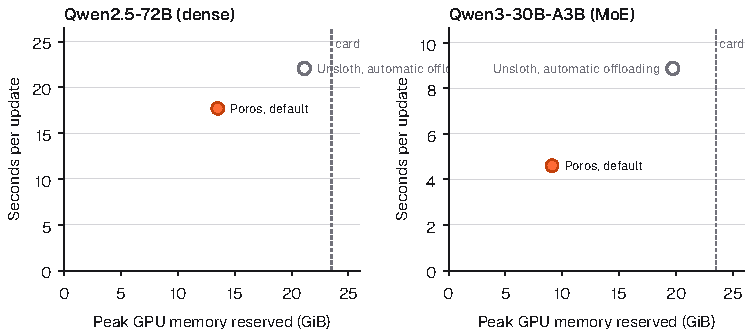
\includegraphics[width=\textwidth]{figure1_h2h.pdf}
\captionsetup{type=figure}
\caption{Seconds per optimizer update (down is faster) against PyTorch's peak reserved GPU memory (left
is less) for the RTX~4090 head-to-head (\nv{wl.ga} micro-batches of \nv{wl.mb} row of \nv{wl.seq} tokens
per update, Unsloth in deterministic mode): Qwen2.5-72B is from \nv{dense.date} (Poros at \nv{dense.commit} against Unsloth \nv{prev.unsloth.version}), and \nv{moe.model} from \nv{env.unsloth.date} (the release commit against Unsloth \nv{env.unsloth}). Each panel shows
two configurations: Poros's default path (filled orange) and Unsloth's automatic offloading (hollow grey), which keeps the layers that fit on the GPU rather than minimizing GPU memory; on \nv{moe.model}, Unsloth also stored fp32 adapters against Poros's bf16 ones, and with all \nv{prev.moe.unsmin.offloaded} layers offloaded Unsloth \nv{prev.unsloth.version} reserved \nv{prev.moe.unsmin.res.best}\,GiB on \nv{prev.unsloth.date}.
Each point is the median of three runs, and each run's value is the median over its updates after the
initial one. Dashed line: the card's capacity as PyTorch reports it (\nv{card.gib}\,GiB). \Cref{tab:h2h}
lists every value and host memory. On \nv{moe.model}, Unsloth \nv{env.unsloth} ran \nv{moe.unsloth.slower.median} slower per update by median than Unsloth \nv{prev.unsloth.version} did on \nv{prev.unsloth.date} with the same harness and rows; the logs do not show why.\ \nv{fig1.status}}
\label{fig:hero}
\end{minipage}
\vspace{2pt}

% ============================================================================
\section{Introduction}\label{sec:intro}

LoRA freezes a model and trains small low-rank matrices~\cite{hu2021lora}.
QLoRA stores frozen weights in 4-bit NF4 and backpropagates through them (65B fine-tuning on one 48\,GB GPU)~\cite{dettmers2023qlora}.
Common implementations keep frozen weights on the GPU, yet Qwen2.5-72B's 4-bit weights alone exceed a 24\,GB card.
Unsloth~\cite{unsloth} trains it on a 24\,GB GPU by offloading decoder layers to host memory.
Swapping weights and activations between GPU and host is an old idea~\cite{rhu2016vdnn,huang2020swapadvisor,ren2021zero,rajbhandari2021zeroinfinity,pudipeddi2020l2l}.
Each frozen weight is read twice per micro-batch, in the forward and the backward pass, and never written; the trainable state is small.

Poros uses \emph{blockwise residency}: the frozen 4-bit base stays in host memory, or in an SSD file (the \emph{SSD store}) for a mixture-of-experts (MoE) model's experts.
One block of layers moves to the GPU at a time and is recomputed in the backward pass; adapters and optimizer state stay on the GPU.
With gradient accumulation, \emph{block-major accumulation} copies each block once per pass for all micro-batches of an update, so the frozen base crosses the bus twice per update (\cref{sec:blockmajor}).
The sequential schedule copies it twice per micro-batch.
Floating-point addition is non-associative~\cite{goldberg1991floating}; moving computation can change low bits and hide an offloading bug as noise.
Streamed losses, adapters, and optimizer state must be identical to those of the \emph{resident run} on the same hardware and software.
The resident run uses the same Poros configuration with all frozen weights on the GPU and no recomputation (\cref{sec:exact} defines identical and equal).
A violation is a test failure.
A MoE model's expert adapters are bf16 parameters, and PyTorch's AdamW on bf16 weights drops small updates.
Poros steps them with its own optimizer (\cref{sec:expertadamw}).
We make four contributions:
\begin{itemize}
\item \textbf{Design (\cref{sec:design}).}
Poros combines blockwise residency, block-major accumulation (L2L's loop order~\cite{pudipeddi2020l2l} applied to frozen-base QLoRA, with random-number-state restoration), two paths for saved block inputs (the \emph{efficient path} and the \emph{fast path}), and a streamed loader.
It adds MoE expert streaming with the SSD store, an optimizer for bf16 expert adapters, and the Mac backend.

\item \textbf{Exactness (\cref{sec:exact,sec:testing}).}
We state premises under which a streamed run is identical to the resident run.
On the release engine, \code{poros prove} found a streamed run of \nv{prove.model} equal to the resident run on the RTX~4090.
The family gate gave identical adapters across schedules and paths on \nv{fg.n} rows, and dropout-on checks at \nv{do.dropout} were equal on three models.
A resident Qwen2.5-72B run does not fit a 24\,GB GPU, and no resident run of \nv{moe.model} was made.
Their equality with a resident run is argued (\cref{sec:exact}) and was not tested.

\item \textbf{Optimizer (\cref{sec:expertadamw,sec:opt-eval}).}
Poros steps bf16 expert adapters with a keyed stochastic-rounding AdamW rule.
Per update, from the same stored state, its fp32 update agrees with fp32 AdamW to within a rounding ($2^{-24}$ relative) for weights above $2^{-53}$, and within $2^{-77}$ below that at $\beta_1 \le 0.999$.
Its GPU kernels match the CPU reference bit for bit on \nv{st.devices}.
On OLMoE-1B-7B (\nv{olmoe.updates} updates, one run per arm), held-out loss at the end of the run was \nv{olmoe.heldout.new} against \nv{olmoe.heldout.fp32} for fp32 adapters (largest difference \nv{olmoe.maxdiff}; fp32 seed gap \nv{olmoe.seedgap}).

\item \textbf{Evaluation (\cref{sec:eval}).}
On the 24\,GB RTX~4090 workload (\cref{fig:hero,tab:h2h}), Poros's default path reserved \nv{moe.ram.res} against \nv{moe.unsloth.res}\,GiB on \nv{moe.model} versus Unsloth \nv{env.unsloth} (\nv{env.unsloth.date}, automatic layer offloading, deterministic mode); automatic offloading keeps the layers that fit on the GPU, and Unsloth stored fp32 adapters against Poros's bf16 ones.
On Qwen2.5-72B in an earlier session (\nv{dense.date}, Poros at \nv{dense.commit} against Unsloth \nv{prev.unsloth.version}, automatic offloading, deterministic mode), Poros reserved \nv{dense.poros.res} against \nv{dense.unsloth.res}\,GiB; automatic offloading keeps the layers that fit on the GPU rather than targeting its lowest memory.
On \nv{moe.model}, Poros held \nv{moe.ram.host}\,GiB in host memory (\nv{moe.ram.host.procs} processes at peak), whereas Unsloth's process tree peaked at \nv{moe.unsloth.host.few}\,GiB over samples with three or fewer processes with \nv{env.unsloth} and near \nv{prev.moe.unsloth.host.train}\,GiB while training with \nv{prev.unsloth.version} on \nv{prev.unsloth.date} (\cref{sec:moe-eval}).
In that \nv{dense.date} Qwen2.5-72B session (Poros at \nv{dense.commit} against Unsloth \nv{prev.unsloth.version}), peak process-tree host memory (RssAnon plus RssShmem; \cref{sec:setup}) was \nv{dense.poros.host} against \nv{dense.unsloth.host}\,GiB (\nv{dense.poros.vs.host_ram}); \cref{sec:dense,sec:moe-eval} report update times.
Per-update losses on the same rows differed by at most \nv{loss.30b.maxdiff} on \nv{moe.model} (against Unsloth \nv{env.unsloth} on \nv{env.unsloth.date}) and \nv{loss.72b.maxdiff} on Qwen2.5-72B (Poros at \nv{dense.commit} against Unsloth \nv{prev.unsloth.version} on \nv{dense.date}).
On an 8\,GB laptop GPU (\nv{lap.gpu}), a measured run of \code{moe-30b-8gb} trained Qwen3-30B-A3B-Instruct-2507 at rank \nv{lap.rank} on \nv{lap.seq}-token rows at \nv{lap.supd}\,s per update (\cref{sec:laptop}).
A \nv{mac.gib}\,GB M4 Mac fine-tuned Qwen2.5-72B-Instruct; a \nv{m144.steps}-update run of one row of at most \nv{m144.seq} tokens lowered loss on \nv{m144.heldout} held-out rows from \nv{m144.before} to \nv{m144.after} in \nv{m144.min} minutes (\cref{sec:mac}).
\Cref{tab:recipes} lists \nv{rec.n} recipe runs across the three machines, \nv{rec.cert.n} of them certified on their machine as defined in \cref{sec:recipes}.
Every run records held-out loss, \nv{rec.resume.n} ran a stop-and-continue check that ended at the uninterrupted adapter, and preference loss rose in both preference recipes.
\end{itemize}
Every measured number is read by a script from a committed log (\cref{app:logs}).
Every Poros figure comes from the release engine except the Qwen2.5-72B comparison, which is the \nv{dense.date} session (Poros at \nv{dense.commit} against Unsloth \nv{prev.unsloth.version}); that session's \nv{moe.model} figures are cited for Unsloth alone.

\begin{claimbox}
\textbf{What is claimed.}
Under the premises of \cref{sec:exact}, streamed training is identical to the resident run on the same GPU model and software stack, for NF4 on dense models and for NF4 experts with bf16 non-expert weights on MoE models.
On the release engine, \code{poros prove} found streamed and resident runs of \nv{prove.model} equal on the RTX~4090; no resident run was tested at 72B or on \nv{moe.model} (\cref{sec:testing}).
On the 24\,GB RTX~4090 workload (\cref{tab:h2h}), Poros's default path reserved \nv{moe.ram.res} against \nv{moe.unsloth.res}\,GiB on \nv{moe.model} versus Unsloth \nv{env.unsloth} (\nv{env.unsloth.date}, automatic layer offloading, deterministic mode); automatic offloading keeps the layers that fit on the GPU, and Unsloth stored fp32 adapters against Poros's bf16 ones.
On Qwen2.5-72B (\nv{dense.date}, Poros at \nv{dense.commit} against Unsloth \nv{prev.unsloth.version}, automatic offloading, deterministic mode), Poros reserved \nv{dense.poros.res} against \nv{dense.unsloth.res}\,GiB; automatic offloading keeps the layers that fit on the GPU rather than targeting its lowest memory, and the release engine's big-72b run reserved \nv{recipe.res}\,GiB.
Per update, from the same stored state, the expert optimizer's fp32 update agrees with fp32 AdamW to within a rounding for every weight above $2^{-53}$ (the bound of \cref{sec:expertadamw}).\par\smallskip
\textbf{What is not claimed.}
We do not claim identical or equal results with other stacks (PEFT, Unsloth, or an unpatched Hugging Face loop), across GPU models or software versions, or for precisions other than NF4 (dense) or NF4 experts with bf16 non-expert weights (MoE) (\cref{sec:exact,sec:limits}).
We do not claim less host memory than a tool that keeps part of the model on the GPU (\cref{sec:dense,sec:moe-eval,sec:limits}), nor a speed advantage across all Unsloth versions, outside its deterministic mode, or across all workloads (\cref{sec:moe-eval,sec:limits}).
Unsloth streams offloaded layers per micro-batch, so fewer micro-batches per update favor it.
A pre-release comparison on \nv{prev.unsloth.date} in that shape (one micro-batch of eight rows), whose logs are in the benchmark repository, had Unsloth faster; its Poros figures predate the release engine and are not cited.
Models that fit on the GPU were not compared with Unsloth on the release engine (\cref{sec:limits}).
We do not claim that the expert optimizer's stored values equal fp32 AdamW's; each stored value is an unbiased rounding (\cref{sec:expertadamw}).
\end{claimbox}

% ============================================================================

\section{Design}\label{sec:design}

Poros is a Python library on PyTorch~\cite{paszke2019pytorch}, Hugging Face \code{transformers}, PEFT, and \code{bitsandbytes}; we cover single-GPU CUDA and Mac (\cref{sec:mac}).
Every Poros measurement in this report except the \nv{dense.date} Qwen2.5-72B head-to-head ran on one commit, \nv{code.commit} (Poros~\nv{code.version}), which we call \emph{the release engine}.
That Qwen2.5-72B comparison ran Poros at an earlier commit, \nv{dense.commit}, against Unsloth \nv{prev.unsloth.version} (\cref{sec:dense}).
On \nv{moe.model}, that session's log is cited for Unsloth \nv{prev.unsloth.version}'s figures alone, with no Poros numbers.
\Cref{app:logs} indexes the benchmark logs.

\begin{figure}[t]
\centering
% fig_design.tex: Figure 2, blockwise residency and the copy schedule.  No measured numbers.
\begingroup
\sffamily\footnotesize
\tikzset{
  region/.style={draw=lpfg!55,line width=0.5pt,rounded corners=2pt,fill=lppaper},
  blk/.style={draw=lpfg!75,line width=0.4pt,fill=lprule!60,minimum width=2.05cm,minimum height=0.40cm,
              inner sep=0pt,font=\sffamily\scriptsize},
  pre/.style={blk,dashed,fill=white},
  inp/.style={draw=lpmuted,dashed,line width=0.4pt,fill=white,minimum width=2.05cm,minimum height=0.56cm,
              inner sep=0pt,align=center,font=\sffamily\scriptsize,text=lpmuted},
  adapt/.style={draw=lpaccent,line width=0.6pt,fill=lpaccentlt,minimum width=2.05cm,minimum height=0.62cm,
                inner sep=0pt,align=center,font=\sffamily\scriptsize},
  title/.style={font=\sffamily\footnotesize\bfseries,anchor=base west},
  rtitle/.style={font=\sffamily\scriptsize\bfseries},
  note/.style={font=\sffamily\scriptsize,text=lpmuted},
  sq/.style={draw=lpfg!80,line width=0.35pt,minimum size=0.25cm,inner sep=0pt,font=\sffamily\tiny},
  fw/.style={sq,fill=white},
  bw/.style={sq,fill=lpbase!60},
  stay/.style={sq,dashed,draw=lpfg!60,fill=white,text=lpmuted},
  mb/.style={circle,fill=lpfg,inner sep=0pt,minimum size=1.9pt},
  arr/.style={-{Stealth[length=3.6pt,width=3.2pt]},line width=0.55pt,lpfg},
}
\begin{tikzpicture}[x=1cm,y=1cm]
% ===================== (a) where state lives =====================
\node[title] at (0,4.55) {(a) Where state lives};
\node[region,minimum width=2.45cm,minimum height=3.35cm,anchor=south west] (host) at (0,0.95) {};
\node[rtitle,anchor=north] at ($(host.north)+(0,-0.06)$) {Host memory};
\node[note,anchor=north] at ($(host.north)+(0,-0.38)$) {frozen NF4 blocks};
\node[blk] at (1.225,3.33) {$\mathcal{B}_1$};
\node[blk] at (1.225,2.87) {$\mathcal{B}_2$};
\node[font=\scriptsize] at (1.225,2.52) {$\vdots$};
\node[blk] at (1.225,2.10) {$\mathcal{B}_K$};
\node[inp] (hin) at (1.225,1.40) {saved inputs\\[-2pt]efficient path};

\node[region,minimum width=2.45cm,minimum height=3.35cm,anchor=south west,draw=lpfg!80] (gpu) at (3.25,0.95) {};
\node[rtitle,anchor=north] at ($(gpu.north)+(0,-0.06)$) {GPU};
\node[adapt] at (4.475,3.38) {adapters $\theta$\\optimizer state};
\node[blk] (gk) at (4.475,2.64) {$\mathcal{B}_k$ computing};
\node[pre] (gn) at (4.475,2.18) {$\mathcal{B}_{k+1}$ prefetch};
\node[inp] (gin) at (4.475,1.40) {saved inputs\\[-2pt]fast path};

\draw[arr] (2.47,2.64) -- node[note,above,yshift=-1pt] {copy} (3.23,2.64);
\draw[arr,dashed] (2.47,2.18) -- (3.23,2.18);
\draw[{Stealth[length=3pt,width=2.8pt]}-{Stealth[length=3pt,width=2.8pt]},line width=0.4pt,lpmuted,densely dashed]
  (2.27,1.40) -- (3.43,1.40);

\node[region,minimum width=2.45cm,minimum height=0.52cm,anchor=south west,fill=white,draw=lpfg!40,dashed] (ssd) at (0,0.0) {};
\node[note] at (ssd.center) {SSD file: MoE experts};
\draw[lpfg!40,line width=0.4pt,densely dotted] (ssd.north) -- (host.south);
\node[note,anchor=west,align=left] at (3.25,0.26) {no write-back:\\[-1pt]the host copy is the only one};

% ===================== (b) block copies per update =====================
\begin{scope}[xshift=6.35cm]
\node[title] at (0,4.55) {(b) Block copies in one update ($K{=}4$, $\G{=}3$)};
% -- sequential --
\node[rtitle,anchor=base west] at (0,3.95) {Sequential};
\node[note,anchor=base east] at (8.45,3.95) {$2\G K = 24$ copies};
\foreach \g in {0,1,2} {
  \pgfmathsetmacro{\x}{0.13+\g*2.78}
  \foreach \b [count=\i from 0] in {1,2,3,4} {
    \node[fw] at ({\x+\i*0.30},3.55) {\b};
    \node[mb] at ({\x+\i*0.30},3.29) {};
  }
  \foreach \b [count=\i from 4] in {4,3,2,1} {
    \node[bw] at ({\x+\i*0.30},3.55) {\b};
    \node[mb] at ({\x+\i*0.30},3.29) {};
  }
  \node[note] at ({\x+1.05},3.02) {micro-batch \pgfmathparse{int(\g+1)}\pgfmathresult};
}
% -- block-major --
\node[rtitle,anchor=base west] at (0,2.42) {Block-major};
\node[note,anchor=base east] at (8.45,2.42) {\textcolor{lpaccent}{$2K-1 = 7$ copies}};
\foreach \b [count=\i from 0] in {1,2,3,4} {
  \node[fw] at ({0.13+\i*0.62},2.02) {\b};
  \foreach \m in {-1,0,1} {\node[mb] at ({0.13+\i*0.62+\m*0.085},1.76) {};}
}
\foreach \b [count=\i from 0] in {4,3,2,1} {
  \ifnum\b=4
    \node[stay] at ({3.05+\i*0.62},2.02) {\b};
  \else
    \node[bw] at ({3.05+\i*0.62},2.02) {\b};
  \fi
  \foreach \m in {-1,0,1} {\node[mb] at ({3.05+\i*0.62+\m*0.085},1.76) {};}
}
\node[note] at (1.06,1.49) {forward};
\node[note] at (3.98,1.49) {backward, $g=1,\dots,\G$};
% -- legend --
\node[fw] at (0.13,0.62) {};      \node[note,anchor=west] at (0.30,0.62) {forward copy};
\node[bw] at (2.20,0.62) {};      \node[note,anchor=west] at (2.37,0.62) {backward copy};
\node[stay] at (4.45,0.62) {};    \node[note,anchor=west] at (4.62,0.62) {no copy};
\node[mb] at (6.10,0.62) {};      \node[note,anchor=west] at (6.20,0.62) {one micro-batch};
\end{scope}
\end{tikzpicture}
\endgroup

\caption{Blockwise residency.  (a)~The frozen NF4 blocks live in host
memory (or, for MoE experts, in an SSD file) and visit the GPU one at a
time, with the next block prefetched; the adapters and optimizer state
never leave the GPU.  The inputs saved for the backward pass wait in host
memory on the efficient path and on the GPU on the fast path.  (b)~Block
copies in one update with $K=4$ blocks and $\G=3$ micro-batches.  The
sequential schedule copies every block twice per micro-batch; block-major
accumulation copies it twice per update and runs all micro-batches during
each visit (dots).  The last block stays on the GPU between the passes.}
\label{fig:design}
\end{figure}

\subsection{Streaming and recomputing blocks}\label{sec:stream}

Under \emph{blockwise residency}, packed pinned host slabs hold the frozen base (locked memory about weight size), one $m$-layer block visits the GPU at a time, and backward recomputes it (\cref{fig:design}). A dedicated copy stream transfers block $k+1$ (or $k-1$ backward) while block $k$ computes; the compute stream waits on it. Recording that stream per tensor returns released memory to the caching allocator after compute. Frozen GPU weights are bounded by about $2m/L$ of an $L$-layer model, costing one copy per forward and per backward pass plus one extra forward per block.

Block size $m$ (default 4 layers) trades memory for speed without changing results under the premises of \cref{sec:exact}; \code{resident\_blocks} pins chosen blocks.
Embeddings and the LM head stay on the GPU unless \code{offload\_embeddings\_and\_head} moves them to host memory.
When left unset, the check before a run moves the embedding table and the LM head to host memory if it finds GPU memory short, and the run records the reason (\code{offload\_reason}).
\Cref{tab:paths} gives what the \code{big-72b} and \code{big-72b-fast} runs recorded.
Offloaded, both keep their load dtype; lookups widen to fp32 where used (matching a widened table).
The head weight widens where used except under the fused head, where a head whose values are exactly bf16 crosses in bf16 and is multiplied as the fused head of \cref{sec:blockmajor} multiplies it on the GPU.

Each block's forward runs in a custom autograd function saving its input and CPU/CUDA random-number states. Backward reloads the block, restores states in \code{torch.random.fork\_rng}, recomputes with gradients, and calls \code{autograd.grad}. Each adapter parameter's first step gradient is assigned to \code{.grad}; later ones are added in place. PyTorch checkpointing offers this restoration~\cite{pytorch_checkpoint}; Poros needs it per streamed block, as in gradient checkpointing~\cite{chen2016training}.

\subsection{Block-major accumulation}\label{sec:blockmajor}

Under \emph{the sequential schedule}, $\G$ micro-batches stream all $K$ blocks forward and backward ($2\G$ model copies, $2\G K$ blocks per step). \emph{Block-major accumulation} (CUDA default) exchanges the loops (\cref{alg:blockmajor}). Forward copies $\mathcal{B}_k$ once across $\G$ micro-batches (keeping their inputs); the head computes each $1/\G$-scaled loss and gradient. Backward copies each block once to recompute and differentiate micro-batches $1,\dots,\G$ in order. Retaining the last block on the GPU between passes gives $2K-1$ block copies ($2K$ if the head is in host memory).

\begin{algorithm}[t]
\caption{One optimizer step under block-major accumulation (the last block,
which stays resident between the passes, is not shown separately).}
\label{alg:blockmajor}
\small
\begin{algorithmic}[1]
\Require frozen blocks $\mathcal{B}_1,\dots,\mathcal{B}_K$ in host memory; adapters $\theta$ on the GPU; micro-batches $x_1,\dots,x_\G$
\For{$g=1,\dots,\G$}\ $h^{(g)}_0 \gets \mathrm{Embed}(x_g)$\EndFor
\For{$k=1,\dots,K$}\Comment{forward: one copy of each block}
  \State copy $\mathcal{B}_k$ to the GPU (prefetched)
  \For{$g=1,\dots,\G$}
    \State keep $h^{(g)}_{k-1}$ \Comment{on the GPU (fast) or in host memory (efficient)}
    \State $h^{(g)}_k \gets f_k(h^{(g)}_{k-1};\,W_k,\theta_k)$ without a graph
  \EndFor
  \State release $\mathcal{B}_k$
\EndFor
\For{$g=1,\dots,\G$}\ $\ell_g \gets \mathcal{L}(\mathrm{Head}(h^{(g)}_K))$;\ $\delta^{(g)}_K \gets \partial(\ell_g/\G)/\partial h^{(g)}_K$\EndFor
\For{$k=K,\dots,1$}\Comment{backward: one more copy of each block}
  \State copy $\mathcal{B}_k$ to the GPU (prefetched); bring back $h^{(\cdot)}_{k-1}$ if it waited on the host
  \For{$g=1,\dots,\G$}
    \State recompute $f_k(h^{(g)}_{k-1})$ with a graph
    \State $(\delta^{(g)}_{k-1},\,\nabla^{(g)}_{\theta_k}) \gets \mathrm{autograd.grad}(\cdot,\ \delta^{(g)}_k)$;\quad $\theta_k.\mathrm{grad} \mathrel{+}= \nabla^{(g)}_{\theta_k}$
  \EndFor
  \State release $\mathcal{B}_k$
\EndFor
\State optimizer step on $\theta$
\end{algorithmic}
\end{algorithm}

Three details preserve exactness: unconcatenated micro-batches (sequential shapes), adapter gradients accumulated in micro-batch order, and dropout masks matching the sequential schedule. For dense models, walking the sequential order without the model yields each block's generator state, set before forward and recomputation and checked after forward. An unaccounted draw (e.g., the model's own dropout) stops the update before application, and the run continues on the sequential schedule. For MoE, either schedule keys each decoder layer's generator by seed, update, micro-batch, and layer before forward and recomputation; an unkeyed forward layer stops the update before application.

Within a block visit, the fast path reuses dequantized NF4 weights up to a cap and the efficient path dequantizes where used (\cref{sec:paths}); both feed identical dequantized operands.

On NF4 CUDA runs, Poros's fused kernels execute decoder LoRA, SwiGLU, normalization, rotary, attention, residual arithmetic, and head loss by default (\code{fused\_compute: false} restores PEFT). Precisions match PEFT with two exceptions. On dense NF4 CUDA runs, causal attention uses PyTorch's flash kernel on bf16-rounded queries, keys, and values (fp32 accumulation and softmax) where that kernel takes the call, and PyTorch's memory-efficient kernel in fp32 otherwise. MoE models use the memory-efficient kernel. An LM head whose weight values are exactly bf16 multiplies the fp32 hidden state split into a bf16 part and a bf16 remainder, with the two products summed in fp32. Outputs differ from PEFT's modules by ordinary rounding. The CUDA runs of this paper used these kernels where their logs record compute (\cref{tab:paths}); the fp32 arm of the OLMoE optimizer study ran without them (\cref{sec:opt-eval}), and the \code{poros prove} log does not record which ran.

% ---------------------------------------------------------------------------
%  paths.tex: the efficient and fast paths.
%
%  EDIT HERE when the meaning of `path' changes.  This file is
%  the only prose that describes what each path does.  The settings each path
%  resolved to in the measured runs are not typed here: table_paths.tex is
%  generated by launch_results.py from each run's config.resolved.json, so a
%  change in the code shows up in the table without editing this file.  If the
%  definition changes, update the paragraph "What each path sets" and the
%  sentence on the default; the exactness argument (Section 4.5) needs no
%  change as long as every difference between the paths only moves bytes.
% ---------------------------------------------------------------------------
\subsection{Where block inputs wait: the efficient and fast paths}\label{sec:paths}

Block-major accumulation keeps, for every block, the inputs of all $\G$
micro-batches from the forward pass until the backward pass reaches that
block.  On NF4, these inputs are fp32, so they take up to
$\G\cdot K\cdot b\cdot s\cdot d\cdot 4$ bytes for micro-batches of $b$ rows
of $s$ tokens and hidden size $d$.  The bound grows linearly with the
number of tokens in a step and with $K$, so it is largest at block size 1.

The configuration key \code{path} selects the training loop.  Two of its
values use block-major accumulation and differ in where these inputs wait.
On the \emph{fast} path, they stay on the GPU, and each block's dequantized
NF4 weights are kept for all its micro-batches (\cref{sec:blockmajor}).  On
the \emph{efficient} path (the default), each input is copied to host
memory on a side stream as soon as the block that reads it has run.  It is
copied back on another stream one block ahead of its backward, so the copy
overlaps computation.  The host buffers are page-locked slabs allocated once
and reused in every update.  Where the host refuses to page-lock memory, as
some virtualized hosts do, the inputs go to a reused pool of ordinary
memory.  By default, this pool is capped at half the host memory free when
the first page-lock is refused; copies from ordinary memory block the host
thread.  Past either cap, the inputs stay on the GPU.  The efficient path
therefore trades GPU memory for host memory and PCIe traffic, and the fast
path does the reverse.
The third value, \code{sequential}, selects the sequential schedule (not a block-major path) and runs one micro-batch at a time through every block.
It is slower, and its peak GPU memory can be lower than that of the efficient path.
Both paths and the sequential schedule give every kernel the same operands and compute the same results (\cref{sec:corollaries}); they differ in where the block inputs wait and in how often the frozen weights cross the bus.

\paragraph{What each path sets}
In the measured runs, the two paths ran with the settings in \cref{tab:paths}.
Those settings come from the \code{big-72b} (efficient path) and \code{big-72b-fast} (fast path) runs on the RTX~4090, as each run's resolved configuration recorded them.

% Generated by launch_results.py -- do not edit.
\begin{table}[tbp]
\centering
\caption{What each path ran with in the \code{big-72b} (efficient) and \code{big-72b-fast}
(fast) recipes on the RTX~4090, as each run's resolved configuration recorded it.}
\label{tab:paths}
\small
\begin{tabular}{@{}lcc@{}}
\toprule
\tabhead{Setting} & \tabhead{efficient} & \tabhead{fast} \\
\midrule
Path the run recorded (no fallback) & \nvc{paths.eff.ran_path} & \nvc{paths.fast.ran_path} \\
Block size (layers) & \nvc{paths.eff.block_size} & \nvc{paths.fast.block_size} \\
Blocks kept on the GPU & \nvc{paths.eff.resident_blocks} & \nvc{paths.fast.resident_blocks} \\
Embedding and head in host memory & \nvc{paths.eff.offload_embeddings_and_head} & \nvc{paths.fast.offload_embeddings_and_head} \\
Dequantization cache (MiB; 0: off) & \nvc{paths.eff.nf4_dequant_cache_mb} & \nvc{paths.fast.nf4_dequant_cache_mb} \\
Fused compute & \nvc{paths.eff.fused_compute} & \nvc{paths.fast.fused_compute} \\
Expandable allocator segments & \nvc{paths.eff.cuda_expandable_segments} & \nvc{paths.fast.cuda_expandable_segments} \\
Host memory for block inputs and blocks & \nvc{paths.eff.host_staging} & \nvc{paths.fast.host_staging} \\
\bottomrule
\end{tabular}
\end{table}



\subsection{Loading}\label{sec:loader}

Standard \code{transformers}/\code{bitsandbytes} NF4 loading quantizes onto the GPU, requiring the model to fit.
Poros's default streamed loader reads one tensor at a time, quantizes it on the GPU, and moves it to host memory.
In the \nv{dense.date} Qwen2.5-72B head-to-head (Poros at \nv{dense.commit} against Unsloth \nv{prev.unsloth.version}; \cref{sec:dense}), it reserved at most \nv{dense.poros.load.res}\,GiB of GPU memory and took \nv{dense.poros.load.s}\,s.
Poros falls back to standard loading for checkpoints unreadable per tensor (transforms beyond renames, or tensors the model has no place for); other errors stop loading.
For dense models, the streamed loader quantizes each tensor with \code{bitsandbytes} on the GPU as the standard loader does; byte equality of the two loaders is argued and was not measured on the release engine.
MoE experts are quantized differently (\cref{sec:moe}).

\subsection{Mixture-of-experts models and the SSD store}\label{sec:moe}
Attention and dense parts stream by block; experts stream one at a time from host memory (one layer plus a look-ahead slice on the GPU).
After the initial update, a device cache retains experts across updates (default: one layer on the efficient path, or what fits in unused GPU memory up to \code{moe\_expert\_cache\_gib} on the fast path).
During loading, Poros quantizes routed experts one tensor at a time to the \code{bitsandbytes} NF4 format with double quantization using its own PyTorch implementation; attention, norms, router, and embeddings stay bf16.
Quantization runs on the training GPU by default and on the CPU otherwise.
The code documents that both devices produce the same bytes, which was not measured here.
Streamed and resident MoE runs read the same quantized expert bytes; we claim no comparison of those bytes with the CUDA quantization of \code{bitsandbytes}.
LoRA adapts routed experts' gate, up, and down projections with bf16 adapters and gradients, stepped by the optimizer of \cref{sec:expertadamw}; routers, attention, and shared experts stay frozen.
Supported families are Qwen3-MoE, OLMoE, Qwen2-MoE, DeepSeek-V2, Qwen3.5-MoE, and Gemma~4-MoE.
The family gate (\cref{sec:testing}) passes on \nv{fg.moe.families} among its \nv{fg.n} rows, and the head-to-head and recipes train \nv{moe.model}.

Hugging Face's \code{index\_add\_} loop accumulates with unordered atomics. Poros stable-sorts (token, slot) pairs by expert, writes weighted expert outputs to dedicated rows by index assignment, and sums each token's slots in fixed order. Routing runs once per forward, reused in recomputation; a stable top-$k$ replaces routers whose top-$k$ leaves ties to the kernel. There is no capacity limit, token dropping, or auxiliary loss. Where every layer qualifies, experts default to Poros's bf16 fused Triton kernels over exact per-expert rows. Every Poros run of the head-to-head on \nv{moe.model} recorded the fused expert kernels (\cref{sec:moe-eval}). The fp32 arm of the OLMoE optimizer study ran the reference expert compute because the fused kernels require bf16 adapters (\cref{sec:opt-eval}). Otherwise, reference execution runs padded batched multiplications in power-of-two buckets; single-batch grouping (\code{moe\_expert\_grouping: single}) changes multiplication shapes and is argued to compute different bits (\cref{sec:corollaries}).
\paragraph{The SSD store}\label{sec:ssd}
With \code{store: ssd}, \emph{the SSD store} keeps NF4 experts in a 4\,KiB-aligned slab file indexed by 64-bit BLAKE2b per-slab checksums. A thread pool reads slabs via \code{O\_DIRECT} into a page-locked ring (at most 4\,GiB default) for GPU copy; an optional host cache (e.g., \code{store\_options: \{cache: 4G\}}) retains them. Fixed layer order lets backward read forward's experts and uses the prior pass to predict next-layer experts for read-ahead. Each slab is checksum-checked on first read, so the store returns the RAM store's bytes or fails. The first run writes the file; later runs reuse it while checkpoint, layout, quantization, and library versions match, skipping checkpoint expert tensors.
\subsection{Expert adapters and their optimizer}\label{sec:expertadamw}
A MoE model's expert LoRA adapters are bf16 parameters because the fused expert kernels read them in bf16, and at \nv{moe.model}'s expert-adapter size fp32 copies do not fit the small machines Poros targets.
PyTorch's AdamW on bf16 parameters drops any update smaller than half a bf16 unit in the last place of the weight, and its second moment cannot move when $(1-\beta_2)$ times the gap falls below bf16 resolution, so it only ratchets up.

Poros steps bf16 expert adapters with rule \code{poros.expert-adamw.v4}.
The forward pass reads the nearest bf16 to the weight, and every value the optimizer stores is an unbiased keyed rounding of its fp32 value.
Per element, the bf16 parameter $h$ is the fp32 weight $w$ rounded to nearest (ties to even), and a bf16 remainder $l$ stores $w - h$ rounded stochastically to bf16, so $h + l$ is exact in fp32 with expectation $w$.
The first moment $m$ and second moment $v$ are stored as bf16 stochastic roundings of their fp32 values.
At update $t$ with gradient $g$, learning rate $\eta$, weight decay $\lambda$, and denominator offset $\varepsilon$, each step computes PyTorch's decoupled AdamW update from $h + l$ using unrounded fp32 $m_1$ and $v_1$, with every operation a single correctly rounded IEEE fp32 operation and no fused multiply-add:
\begin{align*}
m_1 &= m + (1 - \beta_1)(g - m), &
v_1 &= \beta_2 v + (1 - \beta_2)\, g \cdot g, \\
w_d &= (h + l)(1 - \eta \lambda), &
d &= \sqrt{v_1} / \sqrt{1 - \beta_2^t} + \varepsilon, \\
w' &= w_d + \bigl(-\eta / (1 - \beta_1^t)\bigr)\, m_1 / d.
\end{align*}
The optimizer then stores $h' = \mathrm{RN}_{\mathrm{bf16}}(w')$, $l' = \mathrm{SR}_{\mathrm{bf16}}(w' - h')$, $m' = \mathrm{SR}_{\mathrm{bf16}}(m_1)$, and $v' = \mathrm{SR}_{\mathrm{bf16}}(v_1)$, where $\mathrm{RN}_{\mathrm{bf16}}$ rounds to nearest bf16 (ties to even) and $\mathrm{SR}_{\mathrm{bf16}}$ rounds stochastically to bf16.
A flush map $F$ replaces every input and result of magnitude at most $2^{-126}$ (the smallest normal fp32, subnormals, and zeros) with $+0$, so a device that flushes subnormals computes the same bits.
Mixed-precision training ordinarily holds fp32 master weights~\cite{micikevicius2018mixed}, and stochastic rounding keeps low-precision updates unbiased~\cite{gupta2015deep,zamirai2020revisiting}.
Here the fp32 weight is held as two bf16 values, and the rounding is keyed rather than drawn from a generator.
Per expert-adapter parameter, the GPU holds five bf16 tensors (weight, gradient, $m$, $v$, and remainder): 10 bytes against 16 bytes for fp32 weight, gradient, and moments.

Each stored value takes 16 fresh random bits per update, with three independent draws per element ($v$, $m$, and remainder).
The bits are a pure function of the run seed, the update, the parameter's name, the draw, and the element's index.
A BLAKE2b key per update, parameter, draw, and block of $2^{21}$ elements supplies two coefficients $a$ and $b$, and an element at offset $x$ in its block takes bits $((a x + b) \bmod 2^{36}) \gg 20$.
This multiply-add-shift hash~\cite{dietzfelbinger1996universal} makes each element's rounding unbiased and any two elements in a block independent.
CPU, CUDA, and Mac GPUs draw the same bits, and no PyTorch random generator is read or moved, so dropout masks and data order do not change.
Because the step is elementwise, its result does not depend on chunking, parameter order, or a stop and resume; runs repeat.

A CPU reference defines the rule using PyTorch's basic operations, with square root and division corrected to the correctly rounded IEEE fp32 result.
On CUDA a Triton kernel (floating-point fusion disabled, correctly rounded square root and division) and on a Mac a Metal kernel (floating-point contraction off, exact fp32 square root and division built from $+$, $-$, $\times$, and $\mathrm{fma}$, and integer bf16 rounding) compute the same function.
Each kernel uses one launch per tensor and reads and writes each element once.
At construction, the optimizer probes the device kernel against the reference over inputs exercising every operation (including products at $2^{-126}$ and a weight on a bf16 tie) and uses the kernel only if every bit agrees.
Otherwise it runs the reference (in fp64 on CUDA, on the CPU on a Mac).
The optimizer refuses \code{adam\_epsilon} below $2^{-39}/\sqrt{1-\beta_2}$, a learning rate above $1$, and float16 trainable tensors (bf16 and fp32 only).
Any fp32 parameters among bf16 ones get PyTorch's AdamW math with fp32 state and no remainder, while a dense run whose trainable tensors are all fp32 keeps PyTorch's AdamW unchanged.
Every checkpoint records the rule name in \code{optimizer.json}; resuming from optimizer state written by an older rule is refused, though the adapter weights still load to start a new run.

The flush map $F$ is where the rule parts from fp32 AdamW.
Every value $F$ zeroes has magnitude at most $2^{-126}$, and a term dropped from a weight's update is such a value divided by $d \ge \varepsilon$ (or scaled by the step before that division).
With $\varepsilon \ge 2^{-39}/\sqrt{1-\beta_2}$ and $\eta \le 1$, a dropped term moves a weight by at most $2^{-126}/\varepsilon \le 2^{-87}$, or by $\eta/(1-\beta_1^t)$ times $2^{-87}$ when a flushed $g$ or $m_1$ would have been scaled by the step.
That difference is under $2^{-77}$ per update at $\beta_1 \le 0.999$ (larger only at a $\beta_1$ closer to $1$, early in a run).
Per update, the fp32 weight $w'$ that the rule computes before rounding therefore agrees with fp32 AdamW to within a rounding ($2^{-24}$ relative) for every weight above $2^{-53}$ in magnitude, and within $2^{-77}$ absolute below that.
What is stored is then an unbiased rounding of that fp32 value, not the fp32 value itself.
By design, weights and moments within a bf16 step of $2^{-126}$ are not covered: stochastic rounding can store $2^{-126}$ and the next step reads it as zero, giving a bias of at most about $1.2 \times 10^{-38}$ there.
\Cref{sec:opt-eval} tests the kernels against the reference and the rule against fp32 adapters.


\subsection{On a Mac}\label{sec:macdesign}
Because a Mac's CPU and GPU share one memory pool, layers reach the GPU without copying.
Poros holds frozen layers in memory (\code{store=ram}) or reads each layer's 4-bit copy from a drive (\code{store=ssd}).
The 4-bit copy uses Poros's own implementation of the NF4 format with double quantization (the same code as MoE expert quantization in \cref{sec:moe}).
The Mac runs (\cref{sec:mac}) trained one row per update at block size 1 on the sequential schedule, without CUDA fused kernels or \code{bitsandbytes}.
The reader submits queued GPU work before waiting on a read so the read overlaps that work.
Peak memory on the Mac is the process's peak as each run's log records it.
% ============================================================================
\section{Why streaming does not change the result}\label{sec:exact}

\subsection{What equal means and the premises}

\begin{definition}[Identical and equal runs]
Two runs are \emph{identical} if their losses (and gradient norms, where
recorded) compare equal at every optimizer step and every final adapter
tensor has the same bytes.
Poros checks adapter tensors with a SHA-256 digest over each tensor's
name, dtype, shape, and raw bytes, which distinguishes $+0$ from $-0$.
Two runs are \emph{equal} if their losses (and gradient norms, where
recorded) compare equal as floating-point numbers at every optimizer step
and every compared tensor (each final adapter tensor, and each recorded
adapter-gradient and optimizer-state tensor) passes \code{torch.equal}
(same shape, every element equal).
Because \code{torch.equal} counts $+0$ and $-0$ as equal, \emph{equal}
is the weaker check.
\end{definition}

The \emph{resident run} is the same Poros configuration with every frozen
weight on the GPU and no recomputation; it differs from the streamed run
only in where frozen weights are stored and when values are computed.
Comparisons fix one GPU model, one software stack (driver, CUDA, PyTorch,
\code{transformers}, PEFT, and \code{bitsandbytes} versions), and the
determinism settings below.

Poros enables \code{torch.use\_deterministic\_algorithms(True)}, disables
cuDNN autotuning, and fixes the cuBLAS workspace
(\code{CUBLAS\_WORKSPACE\_CONFIG=:4096:8})~\cite{pytorch_repro}.
Outside the fused attention, Poros restricts PyTorch's scaled dot-product
attention to its math implementation.
The fused attention calls PyTorch's flash or memory-efficient kernel
(\cref{sec:blockmajor}); \cref{p:det} includes that their backward passes
are deterministic under these settings, and the repeat and path gates are
consistent with this.
On NF4 CUDA runs, every Poros path and schedule runs the same fused
kernels (\cref{sec:blockmajor}), so the argument applies to them as to
PEFT's modules.
Under these settings, we rely on three premises.

\begin{premise}[Kernel determinism]\label{p:det}
A kernel launch writes bytes that are a function of the bytes it reads
and of the shapes, strides, dtypes, and alignment of its operands.
It does not depend on timing, on other streams, or on the absolute
addresses of its operands.
The backward pass through a recorded autograd graph is a deterministic
function of the graph, the tensors it saved, and the incoming gradient.
\end{premise}

\begin{premise}[Graph mode]\label{p:grad}
A block's forward computes the same bytes whether or not autograd records
it.
\end{premise}

\begin{premise}[Same frozen bytes]\label{p:bytes}
Whenever a kernel in the streamed run reads a frozen weight, it reads the
bytes that the corresponding kernel of the resident run reads.
\end{premise}

\Cref{p:det} motivates the determinism settings: PyTorch uses a
deterministic algorithm or raises an error where it knows of none, and
timing-based autotuning is off.
PyTorch's caching allocator rounds every block to a multiple of 512 bytes
within segments that \code{cudaMalloc} aligns to at least 256 bytes.
Alignments tested by kernels (typically 16 bytes) therefore depend only
on a tensor's offset within its storage, which both runs share.
PyTorch's autograd engine orders ready nodes on a device by sequence
numbers assigned in forward creation order.
A block's backward thus executes the same kernels in the same order
whether it is part of one large graph or recomputed on its own.
We expect \cref{p:grad} to hold because the forward runs the same
operators in both modes and no attention kernel depends on recording
mode; \cref{sec:testing} tests it.
\Cref{p:bytes} is a property of Poros's storage paths and is argued in
\cref{sec:corollaries}.

\subsection{The sequential schedule is identical to the resident run}

\begin{proposition}\label{prop:seq}
Suppose \cref{p:det,p:grad,p:bytes} hold, the two runs start with
identical adapters, optimizer state, and random-number state, and each
block's random-number state is restored before its recomputation.
Then the sequential schedule is identical to the resident run, for any
block size.
\end{proposition}

\begin{proof}
By induction over optimizer steps, then over micro-batches within a step.
Suppose that at the start of a step the adapters, the optimizer state,
and the global random-number state are identical in both runs; this holds
before the first step by assumption.

\emph{Forward.}
Block $k$ computes $h_k=f_k(h_{k-1};W_k,\theta_k,r_k)$, where $r_k$ is
the random-number state at the block's start.
If $h_{k-1}$ is identical in both runs, then so are $W_k$ (\cref{p:bytes}),
$\theta_k$ (the induction hypothesis), and $r_k$.
The random-number state is identical because both runs make the same draws
in the same order; in the streamed run, recomputations happen inside
\code{fork\_rng}~\cite{pytorch_checkpoint}, which restores the global
state on exit.
By \cref{p:det,p:grad}, $h_k$ is identical.
The embedding output starts the induction and the loss ends it.

\emph{Backward.}
The resident run's backward through block $k$ applies the backward
kernels of the block's recorded graph to the incoming gradient $\delta_k$
and to the tensors the forward saved.
The streamed run restores $r_k$ and recomputes the forward from the saved
$h_{k-1}$ with the graph recorded.
By the forward argument and \cref{p:det}, it records the same graph with
the same saved tensors.
If $\delta_k$ is identical, \cref{p:det} gives identical gradients for
$h_{k-1}$ and for $\theta_k$.
The gradient of the scaled loss with respect to $h_K$ comes from the same
head graph in both runs, which starts the induction from $k=K$ down.
Within a block, a tensor used more than once (such as the residual
stream) receives its contributions in the order fixed by the graph.
Across blocks, the only shared tensor that receives a gradient is the
block boundary $h_{k-1}$, which feeds only block $k$.
Shared tensors without gradients, such as the attention mask and the
rotary tables, are identical by the forward argument.

\emph{Accumulation and update.}
Each adapter parameter belongs to one block and is used once per
micro-batch, so it receives one gradient per micro-batch.
In both runs these $\G$ gradients reach its \code{.grad} in micro-batch
order, the first by assignment and the rest by elementwise addition.
Elementwise IEEE~754 addition of identical operands in the same order
gives identical bytes~\cite{goldberg1991floating}.
Gradient clipping and PyTorch's AdamW then read identical gradients and identical state, so they write identical adapters and state.
The expert optimizer (\cref{sec:expertadamw}) is an elementwise function of the stored values, seed, update, parameter name, and element index, so it also writes identical adapters and state.
This completes the induction.
\end{proof}

\subsection{Block-major accumulation is identical to the sequential schedule}

\begin{proposition}\label{prop:bm}
Under \cref{p:det,p:grad,p:bytes}, with no random draw in the forward
pass (LoRA dropout 0 and no dropout of the model's own), block-major
accumulation is identical to the sequential schedule, and therefore, by
\cref{prop:seq}, to the resident run.
\end{proposition}

\begin{proof}
Index the kernel launches of one step by $(g,k,\phi)$: micro-batch $g$,
block $k$, and phase $\phi\in\{\text{forward},\text{backward}\}$, plus
the head launches of each micro-batch.
The launches of $(g,k,\phi)$ read three kinds of data.
First, they read activations and gradients of micro-batch $g$, which are
written only by $(g,k-1,\text{forward})$, $(g,k+1,\text{backward})$, or
the head of $g$.
Second, they read the frozen weights and adapters of block $k$, which no
launch in the step writes.
Third, in the backward phase, they read the gradient accumulators of
$\theta_k$, which only the launches $(g',k,\text{backward})$ for
$g'=1,\dots,\G$ write.
Both schedules respect every dependency of the first kind, so each launch
reads operands produced by the same launches.
Since micro-batches are never concatenated, those operands have the same
shapes.
By \cref{p:det}, each launch writes the same bytes.
The accumulators of $\theta_k$ receive their $\G$ addends in the order
$g=1,\dots,\G$ under both schedules, so they end with the same bytes.
The logged loss is the sum of the $\G$ micro-batch losses in the same
order.
With no random draw in the forward pass, no launch reads the
random-number generator, so the different visiting order has no effect.
\end{proof}

Without generator restoration, the condition on random draws is
necessary because each draw advances a single generator.
The sequential schedule draws the mask of $(g,k)$ after every draw of
micro-batches $1$ to $g-1$.
Block-major accumulation draws it after the masks of blocks $1$ to $k-1$
of every micro-batch, so the masks come from different positions of the
stream.
For dense models, Poros removes this condition by setting the generator
before each $(g,k)$ to the sequential schedule's state, computed by
walking the sequential order (\cref{sec:blockmajor}).
Poros checks the state after each forward pass; an unaccounted draw, such
as the model's own dropout, stops the update and the run continues on the
sequential schedule.
For MoE models, under both schedules, Poros sets the generator before
each layer of each micro-batch to a state keyed by the seed, the update,
$g$, and the layer, so the masks of $(g,k)$ do not depend on block
visiting order.
With these states set, the argument of \cref{prop:bm} applies to the
dropout masks as to every other operand.

\subsection{What leaves the bytes unchanged and what changes them}\label{sec:corollaries}

\Cref{p:bytes} and \cref{prop:seq,prop:bm} cover options that move or
reuse bytes without changing kernel operands or shapes.
\emph{Block size} and \code{resident\_blocks} change GPU weight placement
and where recomputation starts; host-GPU copies are bytewise and
\cref{prop:seq} holds for any block size.
\emph{The path} (\cref{sec:paths}) copies saved block inputs to host
memory and back bytewise.
On dense models, \emph{the streamed loader} (\cref{sec:loader}) quantizes
each tensor with \code{bitsandbytes} on the GPU, as the standard loader
does.
The claim that both loaders produce identical bytes is argued and was not
measured on the release engine.
\emph{MoE experts} are quantized by Poros's own PyTorch implementation of
the \code{bitsandbytes} NF4 format with double quantization, and both a
streamed run and a resident run read those same bytes.
\Cref{p:bytes} for experts rests on both runs using that one
quantization; no comparison with the CUDA quantization of
\code{bitsandbytes} is claimed.
\emph{The SSD store} (\cref{sec:ssd}) returns the RAM store's bytes or
fails a checksum.
\emph{Offloaded embedding and head tables} widen from bf16 to fp32 where
used, which is exact and commutes with row selection.
\emph{The dequantization cache} reuses a deterministic function of NF4
bytes without changing kernel choice.
\emph{Expandable allocator segments} change placement while preserving
512-byte rounding.
The \emph{MoE device cache} keeps experts on the GPU across updates and
skips host-GPU copies.
The expert optimizer's step is elementwise and its rounding bits are keyed by element index, so chunking, parameter order, and block visiting order do not change its output (\cref{sec:expertadamw}).

Four changes alter bits.
MoE expert grouping changes multiplication shapes; because floating-point
summation is order-dependent~\cite{goldberg1991floating}, different
groupings are argued to produce different bits, though each is
deterministic.
A different GPU model or software version may select different kernels,
so the claim holds per GPU model and software stack.
Another implementation of the recipe (PEFT's loop or Unsloth) uses other kernels and operation orders.
On the head-to-head rows (\cref{sec:setup}), per-update losses differed by at most \nv{loss.30b.maxdiff} on \nv{moe.model} (Poros against Unsloth \nv{env.unsloth}, \nv{env.unsloth.date}) and \nv{loss.72b.maxdiff} on Qwen2.5-72B (Poros at \nv{dense.commit} against Unsloth \nv{prev.unsloth.version}, \nv{dense.date}); on \nv{moe.model} the tools also differed in the adapters' dtype (bf16 against fp32) and the \code{transformers} version, and Poros kept its non-expert weights in bf16 (Unsloth's log does not list which of its layers it quantized).
Merged adapter export rounds each merged weight to bf16 once.

\subsection{What was tested on the release engine}\label{sec:testing}
A \emph{gate} runs two fresh processes from one configuration, differing in the mechanism under test alone, and tests whether they are identical or equal.
Because \cref{p:det,p:grad,p:bytes} cannot be proven, gates supply the evidence.
LoRA initializes its $B$ matrices to zero, so half the adapter tensors are trivially identical before an optimizer update; multi-update, gradient, and optimizer-state checks are stronger.

For \cref{prop:seq}, \code{poros prove} on the \nv{prove.gpu} compared streamed and resident runs of \nv{prove.model} over \nv{prove.steps} updates of \nv{prove.seq} tokens.
The streamed run used blocks of \nv{prove.str.bs} layers; the resident run kept all \nv{prove.res.bs} layers on the GPU under ordinary autograd without recomputation.
Every loss, \nv{prove.grads} adapter gradients, \nv{prove.tensors} adapter tensors, and \nv{prove.opt} optimizer tensors were equal (\code{torch.equal}).
Streaming took \nv{prove.str.s}\,s against \nv{prove.res.s}\,s per update and peaked at \nv{prove.str.vram}\,GiB against \nv{prove.res.vram}\,GiB of GPU memory.

For \cref{prop:bm} and the saved-input paths, the family gate passed \nv{fg.checks} checks on \nv{fg.n} architecture rows on the RTX~4090 (downloads not counted), mostly small or truncated models.
A row for Inkling-2, a family 1.0.0 does not support, was refused as intended and is excluded.
On every included row, the sequential schedule, block-major accumulation on both paths, and keeping every block on the GPU inside Poros's blockwise trainer produced one identical adapter digest.
Running the fast path twice gave the same digest on every row, and \nv{fg.resume.models} also passed a stop-and-continue check.
To test dropout restoration at LoRA dropout \nv{do.dropout}, checks compared the sequential schedule against block-major accumulation on the efficient and fast paths for \nv{do.7b.model} and \nv{do.32b.model}, and on the efficient path alone for OLMoE-1B-7B.
Losses, gradient norms, and adapter tensors were equal on \nv{do.7b.model} (\nv{do.7b.steps} updates, \nv{do.7b.tensors} tensors), OLMoE-1B-7B~\cite{olmoe} (\nv{do.olmoe.steps} updates, \nv{do.olmoe.tensors} tensors), and \nv{do.32b.model} (\nv{do.32b.steps} updates, \nv{do.32b.tensors} tensors).
Across the built-in recipe runs, \nv{rec.resume.n} stop-and-continue checks ended at an adapter identical byte for byte to the uninterrupted run's (\cref{sec:recipes}).
On the laptop, the \code{moe-30b-8gb} recipe gave identical adapters across \nv{lap.repeat.runs} runs (\cref{sec:laptop}).

Several parts of the argument were not tested on the release engine.
No streamed-against-resident comparison under ordinary autograd ran above 7B or on any MoE model; the ``every block on the GPU'' arm runs inside Poros's blockwise trainer.
A resident Qwen2.5-72B run does not fit a 24\,GB card, and no resident run of \nv{moe.model} was made.
On those models, the evidence rests on the family gate on smaller models of the same families, the stop-and-continue checks, repeats, and \cref{prop:seq,prop:bm}.
For dense models, byte equality of the streamed and standard loaders is argued (\cref{sec:loader}) and was not tested on the release engine.
Identical runs are claimed per GPU model and software stack, for NF4 on dense models and for NF4 experts with bf16 non-expert weights on MoE models.
\Cref{tab:exact} lists the gates.
% Generated by launch_results.py -- do not edit.
\begin{table}[tbp]
\centering
\caption{Gates on the release engine, commit \nvc{code.commit} (\cref{sec:testing}).  ``Identical'': one
SHA-256 over every adapter tensor's name, dtype, shape and raw bytes, and every loss equal.
``Equal'': the loss at every step and every compared tensor equal under \code{torch.equal}, which
counts $+0$ and $-0$ as equal.  4060L: the RTX~4060 Laptop GPU.}
\label{tab:exact}
\footnotesize
\setlength{\tabcolsep}{3pt}
\begin{tabular}{@{}>{\raggedright\arraybackslash}p{3.1cm}>{\raggedright\arraybackslash}p{2.4cm}>{\raggedright\arraybackslash}p{2.6cm}lr>{\raggedright\arraybackslash}p{3.2cm}@{}}
\toprule
\tabhead{Run under test} & \tabhead{Reference} & \tabhead{Model} & \tabhead{GPU} & \tabhead{Steps} & \tabhead{Result} \\
\midrule
\multicolumn{6}{@{}l}{\emph{Streamed against the whole model on the GPU under ordinary autograd}} \\
\code{poros prove}: streamed, blocks of \nvc{prove.str.bs} layers & resident (\nvc{prove.res.bs} layers, ordinary autograd) & \nvc{prove.model} & 4090 & \nvc{prove.steps} & equal: losses, \nvc{prove.grads} gradients, \nvc{prove.tensors} adapter and \nvc{prove.opt} optimizer tensors \\
\addlinespace
\multicolumn{6}{@{}l}{\emph{Between Poros schedules and paths}} \\
Sequential; block-major on the efficient and fast paths & every block on the GPU (in Poros's trainer) & the family gate's \nvc{fg.n} rows & 4090 &  & identical (one digest per row) \\
Block-major, efficient and fast paths, dropout \nvc{do.dropout} & sequential & \nvc{do.7b.model} & 4090 & \nvc{do.7b.steps} & equal: losses, gradient norms, \nvc{do.7b.tensors} adapter tensors \\
Block-major, efficient path, dropout \nvc{do.dropout} & sequential & OLMoE-1B-7B & 4090 & \nvc{do.olmoe.steps} & equal: losses, gradient norms, \nvc{do.olmoe.tensors} adapter tensors \\
Block-major, dropout \nvc{do.dropout} & sequential & \nvc{do.32b.model} & 4090 & \nvc{do.32b.steps} & equal: losses, gradient norms, \nvc{do.32b.tensors} adapter tensors \\
\addlinespace
\multicolumn{6}{@{}l}{\emph{Repeats and resumption}} \\
Fast path, run again & fast path & the family gate's \nvc{fg.n} rows & 4090 &  & identical \\
Stopped and continued & uninterrupted & \nvc{fg.resume.models} & 4090 &  & identical \\
Stopped and continued & uninterrupted & \nvc{rec.resume.n} recipe runs & all &  & identical adapter \\
\code{moe-30b-8gb}, run again & \nvc{lap.repeat.runs} runs & Qwen3-30B-A3B & 4060L & \nvc{lap.updates} & identical \\
\bottomrule
\end{tabular}
\end{table}


% ============================================================================
\section{Evaluation}\label{sec:eval}
\subsection{Setup}\label{sec:setup}

RTX~4090 head-to-head runs used one machine: \nv{env.gpu} (\nv{env.gpu.mib}\,MiB driver, \nv{card.gib}\,GiB PyTorch), \nv{env.cpu}, \nv{env.host.gib}\,GiB host memory, \nv{env.os}, driver \nv{env.driver}.
For the \nv{env.unsloth.date} \nv{moe.model} comparison, Poros (commit \nv{code.commit}, \nv{code.version}, the release engine, fused kernels on as each run recorded) used PyTorch \nv{env.torch}, CUDA \nv{env.cuda}, \code{transformers} \nv{env.transformers}, PEFT \nv{env.peft}, and \code{bitsandbytes} \nv{env.bnb}.
Unsloth \nv{env.unsloth}~\cite{unsloth} (the newest version on PyPI on \nv{env.unsloth.date}) ran in its own environment (\code{transformers} \nv{env.unsloth.transformers}, PEFT \nv{env.unsloth.peft}, same PyTorch and \code{bitsandbytes}).
The Qwen2.5-72B comparison ran on \nv{dense.date}, Poros at commit \nv{dense.commit} against Unsloth \nv{prev.unsloth.version} (\cref{sec:dense}).
Under automatic offloading, its \code{offload\_layers} option keeps the decoder layers that fit on the GPU and streams the offloaded ones from host memory for every micro-batch.
The harness pinned no package versions; each tool ran on the \code{transformers} version its own requirements resolve to.
Unsloth \nv{env.unsloth}, like \nv{prev.unsloth.version} on \nv{prev.unsloth.date}, caps \code{transformers} at \nv{env.unsloth.tf.cap}, so \code{pip} resolved \nv{env.unsloth.transformers} on both dates; Poros \nv{code.version} requires \nv{env.tf.req}, which resolved to \nv{env.transformers}.

Qwen2.5-72B~\cite{qwen25} (\nv{dense.layers} dense decoder layers, Qwen license) has 4-bit weights that alone exceed the card's capacity.
\nv{moe.model}~\cite{qwen3} is a mixture-of-experts model (\nv{moe.layers} decoder layers, \nv{moe.experts} routed experts per layer); neither tool ran with the whole model on the GPU.
Both tools loaded the same local bf16 snapshot and quantized at load with double quantization and bf16 compute.
On Qwen2.5-72B, both quantized the linear layers to NF4. On \nv{moe.model}, Poros quantized the routed experts to NF4 and kept attention, norms, router and embeddings in bf16; Unsloth's load used the same NF4 settings; its log does not list which of its layers it quantized.

\Cref{tab:setup} lists the recorded head-to-head settings: LoRA rank \nv{wl.rank}, \nv{wl.updates} updates of \nv{wl.ga} micro-batches of \nv{wl.mb} row of \nv{wl.seq} tokens, on \nv{wl.rows} rows of OpenAssistant conversations (oasst1)~\cite{kopf2023oasst}.
Both tools read identical token rows in identical order (matching SHA-256) with expandable allocator segments.
On Qwen2.5-72B, both tools adapted decoder attention and MLP projections (Poros \nv{dense.adapter.dtype} adapters, Unsloth \nv{dense.unsloth.adapter.dtype}).
On \nv{moe.model}, both adapted every routed expert's fused gate-and-up and down projections.
Poros's expert adapters are \nv{moe.adapter.dtype} parameters (the experts' compute dtype) stepped by the optimizer of \cref{sec:expertadamw}, and Unsloth's are \nv{moe.unsloth.adapter.dtype}.
The harness also passed attention output projections as targets for Unsloth (not for Poros) and froze them (\nv{moe.unsloth.oproj} zero-held parameters); Unsloth does not require those adapters, and any effect of them on its run time was not isolated.
Poros's \nv{moe.trainable} trainable expert-adapter parameters, gradients, both moments, and remainders take a computed \nv{moe.adapter.state.gib}\,GiB of GPU memory (10 bytes per parameter across five bf16 tensors, not measured).
The harness's record does not name the optimizer Unsloth ran.
Unsloth ran in deterministic mode throughout, which may slow it; no run without that mode was measured.
Over \nv{wl.updates} updates on the same rows (one run each), Poros's logged loss and Unsloth's mean micro-batch loss differed by at most \nv{loss.30b.maxdiff} on \nv{moe.model} (Unsloth \nv{env.unsloth}, \nv{env.unsloth.date}) and \nv{loss.72b.maxdiff} on Qwen2.5-72B (Poros at \nv{dense.commit}, Unsloth \nv{prev.unsloth.version}, \nv{dense.date}).

% Generated by launch_results.py -- do not edit.
\begin{table}[tbp]
\centering
\caption{Settings of the head-to-head runs, as each run recorded them: Poros's resolved configuration
and its run records, and the Unsloth harness's record.  Poros's quantization settings and optimizer
are its code's (\cref{sec:setup,sec:expertadamw}).  The Unsloth record does not store LoRA $\alpha$,
dropout, the optimizer's name or its learning-rate schedule.}
\label{tab:setup}
\footnotesize
\begin{tabular}{@{}>{\raggedright\arraybackslash}p{3.6cm}>{\raggedright\arraybackslash}p{4.6cm}>{\raggedright\arraybackslash}p{4.6cm}@{}}
\toprule
\tabhead{Setting} & \tabhead{Poros} & \tabhead{Unsloth} \\
\midrule
Base model weights & NF4 with double quantization and bf16 compute, quantized at load from the bf16 checkpoint; on \nvc{moe.model} the routed experts only, with attention, norms, router and embeddings in bf16 & the same local snapshot, quantized at load with the same NF4, double-quantization and bf16-compute settings (the session's record; its log does not list which layers it quantized) \\
LoRA rank, $\alpha$, dropout & \nvc{wl.rank}, \nvc{wl.alpha}, \nvc{wl.dropout} & rank \nvc{wl.unsloth.rank} \\
LoRA targets (Qwen2.5-72B) & every linear layer of every decoder layer & \nvc{wl.unsloth.targets} \\
Trainable parameters (Qwen2.5-72B) & \nvc{wl.trainable72} & \nvc{wl.trainable72} \\
LoRA targets (\nvc{moe.model}) & every routed expert's gate and up projection and its down projection & the same, and the attention output projection, held at zero \\
Trainable parameters (\nvc{moe.model}) & \nvc{moe.trainable} & \nvc{moe.trainable} \\
Adapter dtype (Qwen2.5-72B; \nvc{moe.model}) & \nvc{dense.adapter.dtype}; \nvc{moe.adapter.dtype} & \nvc{dense.unsloth.adapter.dtype}; \nvc{moe.unsloth.adapter.dtype} \\
Tokens per row & \nvc{wl.seq} & \nvc{wl.seq} \\
Rows per micro-batch $\times$ micro-batches & \nvc{wl.mb} $\times$ \nvc{wl.ga} & \nvc{wl.mb} $\times$ \nvc{wl.ga} \\
Learning rate, weight decay, clipping & \nvc{wl.lr}, \nvc{wl.wd}, \nvc{wl.clip} & \nvc{wl.unsloth.lr}, \nvc{wl.unsloth.wd}, \nvc{wl.unsloth.clip} \\
Optimizer, schedule, seed & AdamW ($\beta$ \nvc{wl.betas}): PyTorch's on fp32 adapters, \cref{sec:expertadamw}'s on bf16 expert adapters; \nvc{wl.sched}, \nvc{wl.seed} & seed \nvc{wl.unsloth.seed} \\
Data & \nvc{wl.rows} rows of oasst1 & the same rows (one SHA-256) \\
Updates per run & \nvc{wl.updates} & \nvc{wl.updates} \\
Determinism & deterministic algorithms & deterministic mode \\
Gradient checkpointing & per block (recompute) & \nvc{wl.unsloth.gc} \\
Offloading (Qwen2.5-72B) & every block streamed & \nvc{dense.unsloth.offloaded} of \nvc{dense.layers} layers in host memory; input embedding on \nvc{dense.unsloth.embed} \\
Software & PyTorch \nvc{env.torch}, \code{transformers} \nvc{env.transformers}, PEFT \nvc{env.peft}; on Qwen2.5-72B, Poros at \nvc{dense.commit} (which records itself as Poros \nvc{dense.poros.version}) with the same PyTorch, \code{transformers}, PEFT and \code{bitsandbytes} & Unsloth \nvc{env.unsloth}, \code{transformers} \nvc{env.unsloth.transformers}, PEFT \nvc{env.unsloth.peft} (Qwen2.5-72B: Unsloth \nvc{prev.unsloth.version}, \nvc{dense.date}) \\
\bottomrule
\end{tabular}
\end{table}


Each configuration ran three interleaved times in one session.
Update time is a run's median after the initial update (warm-up, Unsloth compilation, Poros expert-cache growth), reported as the three-run median.
\emph{GPU memory} is PyTorch's peak allocated and reserved memory across load and training (GiB, $2^{30}$ bytes).
\emph{Host memory} is peak non-file-backed resident memory (\code{RssAnon} plus \code{RssShmem}, process and children, sampled every \nv{env.sampler.s}\,s, launch to exit), whole-run and during training alone (after load); a sum over forked child processes can count shared pages more than once, so no host-memory ratio is given where a peak sums more than three processes (\cref{sec:moe-eval}).
It excludes reclaimable memory-mapped checkpoint pages; logged VmHWM is not comparable across tools because Unsloth memory-maps checkpoints.
Comparisons set Poros's median against the other tool's fastest run of three for update time and lowest-value run of three for memory (\cref{tab:h2h} prints Unsloth's).
Ratios are reported to one decimal, or as a whole percent under 1.1 times, rounded against Poros (down where Poros is ahead, up where the other tool is ahead).
A difference that rounds to 0\% reads ``the same''.

\subsection{Qwen2.5-72B}\label{sec:dense}

% Generated by launch_results.py -- do not edit.
\begin{table}[tbp]
\centering
\caption{QLoRA on one RTX~4090 (24\,GB) for two models on which Unsloth's automatic offloading
keeps decoder layers in host memory, Unsloth in its deterministic mode.  \nvc{moe.model}: Poros at the release
commit \nvc{code.commit} against Unsloth \nvc{env.unsloth}, the newest version on PyPI on \nvc{env.unsloth.date}.
Qwen2.5-72B: the \nvc{dense.date} session, Poros at its commit \nvc{dense.commit} against Unsloth
\nvc{prev.unsloth.version}, with the same harness and rows (the 72B comparison was not repeated at the release commit).  Automatic offloading keeps the
decoder layers that fit on the GPU, so its reserved memory measures that placement, not its lowest setting.
On \nvc{moe.model}, Unsloth \nvc{env.unsloth} ran \nvc{moe.unsloth.slower.median} slower per update by median
(\nvc{moe.unsloth.slower.best} by its fastest run) than Unsloth \nvc{prev.unsloth.version} did on
\nvc{prev.unsloth.date} with the same harness and rows (\nvc{prev.moe.unsloth.supd.best}\,s at its fastest run,
\nvc{prev.moe.unsloth.res.best}\,GiB reserved); the logs do not show why.  With all
\nvc{prev.moe.unsmin.offloaded} decoder layers in host memory, Unsloth \nvc{prev.unsloth.version} ran at
\nvc{prev.moe.unsmin.supd.best}\,s per update at its fastest run (\nvc{prev.moe.unsmin.supd}\,s median) and reserved
\nvc{prev.moe.unsmin.res.best}\,GiB on that date.  On \nvc{moe.model}, Unsloth stored fp32 adapters and Poros bf16 ones (about
\nvc{moe.adapter.gap.gib}\,GiB if Unsloth's moments were fp32; computed).
$^{*}$Unsloth's host peak on \nvc{env.unsloth.date} sums \nvc{moe.unsloth.host.procs} processes (a sum over forked processes can count
shared pages more than once); over samples with three or fewer it was \nvc{moe.unsloth.host.few}\,GiB.  s/upd.: seconds per
optimizer update (\nvc{wl.ga} micro-batches of \nvc{wl.mb} row of \nvc{wl.seq} tokens), the median over the
updates after the initial one, then the median of three runs.  GPU: peak allocated / peak reserved by PyTorch.
Host: peak host memory that is not file-backed, summed over the process tree, during training / over the whole run.
Memory in GiB.  The last column compares Poros's median with Unsloth's fastest run of three for time and its
lowest-value run of three for memory, given under its row.  Orange rows are Poros.}
\label{tab:h2h}
\footnotesize
\setlength{\tabcolsep}{3.2pt}
\begin{tabular}{@{}>{\raggedright\arraybackslash}p{4.1cm}rccp{3.85cm}@{}}
\toprule
\tabhead{Configuration} & \tabhead{s/upd.} & \tabhead{GPU} & \tabhead{Host} & \tabhead{Speed; reserved GPU memory, against Unsloth} \\
\midrule
\multicolumn{5}{@{}l}{\emph{Qwen2.5-72B}, dense, \nvc{dense.layers} decoder layers} \\
Unsloth, automatic offloading (\nvc{dense.unsloth.offloaded} of \nvc{dense.layers} layers in host memory) & \nvc{dense.unsloth.supd} & \nvc{dense.unsloth.alloc} / \nvc{dense.unsloth.res} & \nvc{dense.unsloth.host.train} / \nvc{dense.unsloth.host} &  \\
\quad its lowest-value run of three & \nvc{dense.unsloth.supd.best} & reserved \nvc{dense.unsloth.res.best} & \nvc{dense.unsloth.host.train.best} / \nvc{dense.unsloth.host.best} & \\
\porosrow Poros, efficient path (default) & \nvc{dense.poros.supd} & \nvc{dense.poros.alloc} / \nvc{dense.poros.res} & \nvc{dense.poros.host.train} / \nvc{dense.poros.host} & \nvc{dense.poros.vs.s_per_step}; \nvc{dense.poros.vs.vram_reserved} \\
\addlinespace
\multicolumn{5}{@{}l}{\emph{\nvc{moe.model}}, mixture of experts, \nvc{moe.layers} decoder layers} \\
Unsloth, automatic offloading (\nvc{moe.unsloth.offloaded} of \nvc{moe.layers} layers in host memory) & \nvc{moe.unsloth.supd} & \nvc{moe.unsloth.alloc} / \nvc{moe.unsloth.res} & \nvc{moe.unsloth.host.train}$^{*}$ / \nvc{moe.unsloth.host}$^{*}$ &  \\
\quad its lowest-value run of three & \nvc{moe.unsloth.supd.best} & reserved \nvc{moe.unsloth.res.best} & \nvc{moe.unsloth.host.train.best}$^{*}$ / \nvc{moe.unsloth.host.best}$^{*}$ & \\
\porosrow Poros, experts in host memory, efficient path (default) & \nvc{moe.ram.supd} & \nvc{moe.ram.alloc} / \nvc{moe.ram.res} & \nvc{moe.ram.host.train} / \nvc{moe.ram.host} & \nvc{moe.ram.vs.s_per_step}; \nvc{moe.ram.vs.vram_reserved} \\
\bottomrule
\end{tabular}
\tabnote{Settings: \cref{tab:setup}; both tools read the same rows in the same order. Comparisons set
Poros's median against the other tool's lowest-value run of three. Ratios are given to one decimal (a whole
percent under 1.1 times), rounded against Poros (down where Poros is ahead, up where the other tool is
ahead); a difference that rounds to 0\% reads ``the same''.}
\end{table}


The Qwen2.5-72B comparison (\cref{tab:setup,tab:h2h,fig:hero}) was not repeated at commit \nv{code.commit}; it comes from the \nv{dense.date} session (Poros at an earlier commit, \nv{dense.commit}, against Unsloth \nv{prev.unsloth.version}, automatic offloading, deterministic mode, same harness, rows, and settings).
Automatic offloading kept the decoder layers that fit on the GPU and offloaded \nv{dense.unsloth.offloaded} of the \nv{dense.layers} layers to host memory, so its reserved memory reflects that placement rather than its floor.
Poros's default efficient path ran at \nv{dense.poros.supd}\,s per update against \nv{dense.unsloth.supd}\,s median (\nv{dense.unsloth.supd.best}\,s fastest run) for Unsloth \nv{prev.unsloth.version} (\nv{dense.poros.vs.s_per_step}).
It reserved \nv{dense.poros.res}\,GiB of GPU memory (\nv{dense.poros.alloc}\,GiB allocated) against \nv{dense.unsloth.res}\,GiB for Unsloth \nv{prev.unsloth.version} (\nv{dense.poros.vs.vram_reserved}).
Those ratios belong to the \nv{dense.date} engine; on the release engine, the big-72b recipe (same efficient path, block size, and layout, differing in the Instruct model, generated data, and a cosine schedule at a higher learning rate) ran at \nv{recipe.supd}\,s per update and reserved \nv{recipe.res}\,GiB (\nv{recipe.alloc}\,GiB allocated).
During its \nv{dense.poros.load.s}\,s load, Poros reserved at most \nv{dense.poros.load.res}\,GiB of GPU memory.

Over the whole run, Poros's efficient path peaked at \nv{dense.poros.host}\,GiB of host memory against \nv{dense.unsloth.host}\,GiB for Unsloth \nv{prev.unsloth.version} (\nv{dense.poros.vs.host_ram}).
During training alone, host memory was \nv{dense.poros.host.train}\,GiB for Poros against \nv{dense.unsloth.host.train}\,GiB for Unsloth \nv{prev.unsloth.version} (\nv{dense.poros.vs.host_ram_train}).
By design, Poros holds the whole NF4 base in host memory throughout, whereas Unsloth keeps layers that fit on the GPU and offloads the remaining layers to the host.

\subsection{Qwen3-30B-A3B}\label{sec:moe-eval}
On \nv{moe.model} (\cref{tab:setup,tab:h2h,fig:hero}), automatic offloading in Unsloth \nv{env.unsloth} (\nv{env.unsloth.date}, deterministic mode) kept the decoder layers that fit on the GPU and offloaded \nv{moe.unsloth.offloaded} of \nv{moe.layers} layers to host memory.
Its reserved GPU memory therefore reflects that policy, not its floor.
Poros's default (efficient path, experts in host memory) reserved \nv{moe.ram.res}\,GiB (\nv{moe.ram.alloc}\,GiB allocated) against \nv{moe.unsloth.res}\,GiB for Unsloth \nv{env.unsloth} (\nv{moe.ram.vs.vram_reserved}).
Part of the reserved-memory gap comes from adapter dtype: Unsloth stored fp32 adapters and Poros stored bf16 ones, accounting for about \nv{moe.adapter.gap.gib}\,GiB at 16 against 10 bytes per parameter if Unsloth ran AdamW with fp32 moments (\cref{sec:expertadamw}; computed, not measured).
With all \nv{prev.moe.unsmin.offloaded} decoder layers in host memory on \nv{prev.unsloth.date}, Unsloth \nv{prev.unsloth.version} ran at \nv{prev.moe.unsmin.supd.best}\,s per update in its fastest run (\nv{prev.moe.unsmin.supd}\,s median) and reserved \nv{prev.moe.unsmin.res.best}\,GiB.

Poros ran at \nv{moe.ram.supd}\,s per update against \nv{moe.unsloth.supd}\,s median (\nv{moe.unsloth.supd.best}\,s fastest run) for Unsloth \nv{env.unsloth} on \nv{env.unsloth.date} (\nv{moe.ram.vs.s_per_step}).
On this workload, Unsloth \nv{env.unsloth} ran \nv{moe.unsloth.slower.median} slower per update by median (\nv{moe.unsloth.slower.best} by its fastest run) than Unsloth \nv{prev.unsloth.version} did on \nv{prev.unsloth.date} with the same harness and rows; the logs do not show why.
On \nv{prev.unsloth.date}, the same harness measured Unsloth \nv{prev.unsloth.version} at \nv{prev.moe.unsloth.supd.best}\,s per update in its fastest run (\nv{prev.moe.unsloth.supd}\,s median) and \nv{prev.moe.unsloth.res.best}\,GiB reserved.
Set against those figures, Poros's \nv{env.unsloth.date} median gives: \nv{moe.ram.vs.prev.s_per_step} (the two were not measured in one session).

Poros keeps the whole 4-bit base (NF4 experts and bf16 non-expert weights) in host memory, peaking at \nv{moe.ram.host}\,GiB (\nv{moe.ram.host.procs} processes in its process tree at peak; \nv{moe.ram.host.train}\,GiB during training).
Unsloth's process tree peaked at \nv{moe.unsloth.host.few}\,GiB with \nv{env.unsloth} over samples with three or fewer processes and near \nv{prev.moe.unsloth.host.train}\,GiB while training with \nv{prev.unsloth.version} on \nv{prev.unsloth.date}.
Its summed process-tree peak was \nv{prev.moe.unsloth.host.best}\,GiB with \nv{prev.unsloth.version} and \nv{moe.unsloth.host}\,GiB with \nv{env.unsloth}, the latter while \nv{moe.unsloth.host.children} child processes existed.
A sum over forked processes can count shared pages more than once, so we report no host-memory ratio on this model.

Experts on an SSD are covered by the certified \code{moe-30b-ssd} recipe (\cref{sec:recipes}).
By design, block-major accumulation copies the frozen base once per pass for all micro-batches, whereas Unsloth streams its offloaded layers for every micro-batch.
Unsloth should therefore gain as micro-batches per update fall.
A pre-release comparison on \nv{prev.unsloth.date} in that shape (one micro-batch of eight rows), whose logs are in the benchmark repository, had Unsloth faster; its Poros figures predate the release engine and are not cited.

\subsection{The expert optimizer}\label{sec:opt-eval}
The optimizer self-test ran on \nv{st.devices}.
On each tested device, keyed bits and stochastic rounding matched the CPU, the construction probe passed, repeated kernel runs gave the same bits, and the optimizer selected the fused kernel.
Each kernel's full update (weight, remainder, $m$, and $v$) matched the CPU reference bit for bit over three AdamW settings and three fed-back updates.
Inputs covered element counts divisible and indivisible by 16, many exponents, both signs, zeros, subnormals, $2^{-126}$, the largest finite values, NaN, and infinities.
For reference, the optimizer step alone over \nv{st.elems} bf16 elements (expert optimizer against PyTorch's AdamW on bf16) took \nv{st.times}.

On the \nv{olmoe.gpu}, we trained OLMoE-1B-7B~\cite{olmoe} for \nv{olmoe.updates} updates at learning rate \nv{olmoe.lr} on the same rows and seed (one run per arm).
OLMoE-1B-7B is small enough for fp32 adapters with the reference expert compute; the fp32 arm cannot use the fused expert kernels, which require bf16.
Comparisons with the fp32 arm therefore include the difference between fused and reference expert computations.
\nvif{olmoe.ctl.unchanged}{%
Three arms ran on the release engine: the expert optimizer, fp32 adapters with PyTorch's fp32 AdamW, and a control using PyTorch's AdamW on the bf16 expert adapters.
The expert optimizer and control arms differed in the optimizer alone.
On the same engine and card, a full training update (median over updates after the initial one) took \nv{olmoe.supd.new}\,s with the expert optimizer against \nv{olmoe.ctl.supd}\,s with the bf16 control.
Averaged over all updates, an update left \nv{olmoe.unchanged.new} of sampled weights unchanged under the expert optimizer, \nv{olmoe.unchanged.fp32} under fp32 adapters, and \nv{olmoe.ctl.unchanged} under the bf16 control.
Starting at update 20, the ratio of the stored second moment to an fp64 average of the same gradients ranged from \nv{olmoe.vratio.new} for the expert optimizer.
For the bf16 control, that ratio was \nv{olmoe.ctl.vratio} at its last update.
At the end of the run, held-out loss was \nv{olmoe.heldout.new} for the expert optimizer, \nv{olmoe.heldout.fp32} for fp32 adapters, and \nv{olmoe.ctl.heldout} for the bf16 control.
That end-of-run difference between the expert optimizer and the bf16 control (\nv{olmoe.heldout.new} against \nv{olmoe.ctl.heldout}) falls within the fp32 two-seed gap (\nv{olmoe.seedgap}).%
}{%
Two arms ran on the release engine: the expert optimizer and fp32 adapters with PyTorch's fp32 AdamW.
Averaged over all updates, an update left \nv{olmoe.unchanged.new} of sampled weights unchanged under the expert optimizer and \nv{olmoe.unchanged.fp32} under fp32 adapters.
Under PyTorch's AdamW on bf16 parameters, an update smaller than half a unit in the last place of a bf16 weight leaves that weight unchanged (\cref{sec:expertadamw}).
Starting at update 20, the ratio of the stored second moment to an fp64 average of the same gradients ranged from \nv{olmoe.vratio.new} for the expert optimizer.
At the end of the run, held-out loss was \nv{olmoe.heldout.new} for the expert optimizer and \nv{olmoe.heldout.fp32} for fp32 adapters.%
}
Across all scored points, the largest held-out difference between the expert optimizer and fp32 adapters was \nv{olmoe.maxdiff}, against a largest gap of \nv{olmoe.seedgap} between two fp32 seeds.



\subsection{An 8\,GB laptop GPU}\label{sec:laptop}
On a laptop (\nv{lap.gpu}, \nv{lap.vram.gib}\,GiB as PyTorch reports it; \nv{lap.host.gib}\,GiB host memory; commit \nv{code.commit}), the measured \code{moe-30b-8gb} run (not certified on this card) trained Qwen3-30B-A3B-Instruct-2507 with experts in the SSD store.
The run used the \nv{lap.path} path; its log records that the check before the run turned the efficient path down on this card.
Before training, a one-update preparation run built the SSD store on the laptop, and the measured run then trained from that store.
It ran \nv{lap.updates} updates at LoRA rank \nv{lap.rank}, using \nv{lap.ga} micro-batches of \nv{lap.mb} row of \nv{lap.seq} tokens per update.

Training took \nv{lap.supd}\,s per update, with \nv{lap.alloc}\,GiB allocated, \nv{lap.res}\,GiB reserved, and \nv{lap.host}\,GiB of peak host memory.
Held-out loss fell from \nv{lap.before} to \nv{lap.after} in one run.
Its stop-and-continue check ended at a byte-identical adapter.
A second full run of the same recipe ended at the same adapter (equal SHA-256 across all \nv{lap.repeat.runs} runs).
The second run's stop-and-continue check also ended at that adapter.
Unsloth was not run on the laptop.

\subsection{Built-in recipes}\label{sec:recipes}

% Generated by launch_results.py -- do not edit.
\begin{table}[tbp]
\centering
\caption{The built-in recipes, one run of each built-in recipe at commit \nvc{code.commit}:
\nvc{rec.cert.n} of the \nvc{rec.n} runs are certified on their machine; $^{\dagger}$: measured, not certified on that
machine (the recipe is certified on another).  Model: -I is -Instruct (-Instruct-2507 for Qwen3-30B-A3B).  $r$: LoRA rank.
$b\times G$: rows per micro-batch $\times$ micro-batches per update.  Tok.: tokens per row.  s/upd.: the median
time per update over updates 2 to the last (every update after the first), as each certification records it.  GPU: PyTorch's peak allocated / reserved GiB; a Mac has one memory
pool, and its row gives the pool's allocated peak.  Host: peak host memory that is not file-backed, GiB
(``pool'' on the Mac).  Path: eff.\ efficient, fast the fast path, seq.\ the sequential schedule.
Held-out: loss of the base model $\to$ the trained adapter on rows the run did not train on (a
preference recipe gives its preference loss).  Resume: the adapter of a run stopped and continued
against the uninterrupted run's (``identical'': the same bytes; ``not run'': the recipe skips the check).}
\label{tab:recipes}
\scriptsize
\setlength{\tabcolsep}{1.2pt}
\resizebox{\linewidth}{!}{%
\begin{tabular}{@{}lllrlrrrllll@{}}
\toprule
\tabhead{Recipe} & \tabhead{Model} & \tabhead{Path} & \tabhead{$r$} & \tabhead{$b\times G$} & \tabhead{Tok.} & \tabhead{Upd.} & \tabhead{s/upd.} & \tabhead{GPU} & \tabhead{Host} & \tabhead{Held-out} & \tabhead{Resume} \\
\midrule
\multicolumn{12}{@{}l}{\emph{RTX 4090}} \\
\code{first-run} & Qwen2.5-0.5B-I & \nvc{rec.r4090.first-run.path} & \nvc{rec.r4090.first-run.rank} & \nvc{rec.r4090.first-run.geo} & \nvc{rec.r4090.first-run.tok} & \nvc{rec.r4090.first-run.upd} & \nvc{rec.r4090.first-run.s} & \nvc{rec.r4090.first-run.gpu} & \nvc{rec.r4090.first-run.host} & \nvc{rec.r4090.first-run.ev} & \nvc{rec.r4090.first-run.res} \\
\code{support} & Qwen2.5-7B-I & \nvc{rec.r4090.support.path} & \nvc{rec.r4090.support.rank} & \nvc{rec.r4090.support.geo} & \nvc{rec.r4090.support.tok} & \nvc{rec.r4090.support.upd} & \nvc{rec.r4090.support.s} & \nvc{rec.r4090.support.gpu} & \nvc{rec.r4090.support.host} & \nvc{rec.r4090.support.ev} & \nvc{rec.r4090.support.res} \\
\code{voice} & Qwen2.5-7B-I & \nvc{rec.r4090.voice.path} & \nvc{rec.r4090.voice.rank} & \nvc{rec.r4090.voice.geo} & \nvc{rec.r4090.voice.tok} & \nvc{rec.r4090.voice.upd} & \nvc{rec.r4090.voice.s} & \nvc{rec.r4090.voice.gpu} & \nvc{rec.r4090.voice.host} & \nvc{rec.r4090.voice.ev} & \nvc{rec.r4090.voice.res} \\
\code{prefer} & Qwen2.5-7B-I & \nvc{rec.r4090.prefer.path} & \nvc{rec.r4090.prefer.rank} & \nvc{rec.r4090.prefer.geo} & \nvc{rec.r4090.prefer.tok} & \nvc{rec.r4090.prefer.upd} & \nvc{rec.r4090.prefer.s} & \nvc{rec.r4090.prefer.gpu} & \nvc{rec.r4090.prefer.host} & \nvc{rec.r4090.prefer.ev} & \nvc{rec.r4090.prefer.res} \\
\code{big-32b} & Qwen2.5-32B-I & \nvc{rec.r4090.big-32b.path} & \nvc{rec.r4090.big-32b.rank} & \nvc{rec.r4090.big-32b.geo} & \nvc{rec.r4090.big-32b.tok} & \nvc{rec.r4090.big-32b.upd} & \nvc{rec.r4090.big-32b.s} & \nvc{rec.r4090.big-32b.gpu} & \nvc{rec.r4090.big-32b.host} & \nvc{rec.r4090.big-32b.ev} & \nvc{rec.r4090.big-32b.res} \\
\code{moe-30b} & Qwen3-30B-A3B-I & \nvc{rec.r4090.moe-30b.path} & \nvc{rec.r4090.moe-30b.rank} & \nvc{rec.r4090.moe-30b.geo} & \nvc{rec.r4090.moe-30b.tok} & \nvc{rec.r4090.moe-30b.upd} & \nvc{rec.r4090.moe-30b.s} & \nvc{rec.r4090.moe-30b.gpu} & \nvc{rec.r4090.moe-30b.host} & \nvc{rec.r4090.moe-30b.ev} & \nvc{rec.r4090.moe-30b.res} \\
\code{moe-30b-ssd} & Qwen3-30B-A3B-I & \nvc{rec.r4090.moe-30b-ssd.path} & \nvc{rec.r4090.moe-30b-ssd.rank} & \nvc{rec.r4090.moe-30b-ssd.geo} & \nvc{rec.r4090.moe-30b-ssd.tok} & \nvc{rec.r4090.moe-30b-ssd.upd} & \nvc{rec.r4090.moe-30b-ssd.s} & \nvc{rec.r4090.moe-30b-ssd.gpu} & \nvc{rec.r4090.moe-30b-ssd.host} & \nvc{rec.r4090.moe-30b-ssd.ev} & \nvc{rec.r4090.moe-30b-ssd.res} \\
\code{moe-30b-8gb} & Qwen3-30B-A3B-I & \nvc{rec.r4090.moe-30b-8gb.path} & \nvc{rec.r4090.moe-30b-8gb.rank} & \nvc{rec.r4090.moe-30b-8gb.geo} & \nvc{rec.r4090.moe-30b-8gb.tok} & \nvc{rec.r4090.moe-30b-8gb.upd} & \nvc{rec.r4090.moe-30b-8gb.s} & \nvc{rec.r4090.moe-30b-8gb.gpu} & \nvc{rec.r4090.moe-30b-8gb.host} & \nvc{rec.r4090.moe-30b-8gb.ev} & \nvc{rec.r4090.moe-30b-8gb.res} \\
\code{big-72b} & Qwen2.5-72B-I & \nvc{rec.r4090.big-72b.path} & \nvc{rec.r4090.big-72b.rank} & \nvc{rec.r4090.big-72b.geo} & \nvc{rec.r4090.big-72b.tok} & \nvc{rec.r4090.big-72b.upd} & \nvc{rec.r4090.big-72b.s} & \nvc{rec.r4090.big-72b.gpu} & \nvc{rec.r4090.big-72b.host} & \nvc{rec.r4090.big-72b.ev} & \nvc{rec.r4090.big-72b.res} \\
\code{big-72b-fast} & Qwen2.5-72B-I & \nvc{rec.r4090.big-72b-fast.path} & \nvc{rec.r4090.big-72b-fast.rank} & \nvc{rec.r4090.big-72b-fast.geo} & \nvc{rec.r4090.big-72b-fast.tok} & \nvc{rec.r4090.big-72b-fast.upd} & \nvc{rec.r4090.big-72b-fast.s} & \nvc{rec.r4090.big-72b-fast.gpu} & \nvc{rec.r4090.big-72b-fast.host} & \nvc{rec.r4090.big-72b-fast.ev} & \nvc{rec.r4090.big-72b-fast.res} \\
\addlinespace
\multicolumn{12}{@{}l}{\emph{RTX 4060 Laptop}} \\
\code{first-run} & Qwen2.5-0.5B-I & \nvc{rec.r4060l.first-run.path} & \nvc{rec.r4060l.first-run.rank} & \nvc{rec.r4060l.first-run.geo} & \nvc{rec.r4060l.first-run.tok} & \nvc{rec.r4060l.first-run.upd} & \nvc{rec.r4060l.first-run.s} & \nvc{rec.r4060l.first-run.gpu} & \nvc{rec.r4060l.first-run.host} & \nvc{rec.r4060l.first-run.ev} & \nvc{rec.r4060l.first-run.res} \\
\code{moe-30b-8gb}$^{\dagger}$ & Qwen3-30B-A3B-I & \nvc{rec.r4060l.moe-30b-8gb.path} & \nvc{rec.r4060l.moe-30b-8gb.rank} & \nvc{rec.r4060l.moe-30b-8gb.geo} & \nvc{rec.r4060l.moe-30b-8gb.tok} & \nvc{rec.r4060l.moe-30b-8gb.upd} & \nvc{rec.r4060l.moe-30b-8gb.s} & \nvc{rec.r4060l.moe-30b-8gb.gpu} & \nvc{rec.r4060l.moe-30b-8gb.host} & \nvc{rec.r4060l.moe-30b-8gb.ev} & \nvc{rec.r4060l.moe-30b-8gb.res} \\
\addlinespace
\multicolumn{12}{@{}l}{\emph{M4, 16 GB}} \\
\code{mac-first-run} & Qwen2.5-0.5B-I & \nvc{rec.m4.mac-first-run.path} & \nvc{rec.m4.mac-first-run.rank} & \nvc{rec.m4.mac-first-run.geo} & \nvc{rec.m4.mac-first-run.tok} & \nvc{rec.m4.mac-first-run.upd} & \nvc{rec.m4.mac-first-run.s} & \nvc{rec.m4.mac-first-run.gpu} & \nvc{rec.m4.mac-first-run.host} & \nvc{rec.m4.mac-first-run.ev} & \nvc{rec.m4.mac-first-run.res} \\
\code{mac-7b} & Qwen2.5-7B-I & \nvc{rec.m4.mac-7b.path} & \nvc{rec.m4.mac-7b.rank} & \nvc{rec.m4.mac-7b.geo} & \nvc{rec.m4.mac-7b.tok} & \nvc{rec.m4.mac-7b.upd} & \nvc{rec.m4.mac-7b.s} & \nvc{rec.m4.mac-7b.gpu} & \nvc{rec.m4.mac-7b.host} & \nvc{rec.m4.mac-7b.ev} & \nvc{rec.m4.mac-7b.res} \\
\code{mac-support} & Qwen2.5-7B-I & \nvc{rec.m4.mac-support.path} & \nvc{rec.m4.mac-support.rank} & \nvc{rec.m4.mac-support.geo} & \nvc{rec.m4.mac-support.tok} & \nvc{rec.m4.mac-support.upd} & \nvc{rec.m4.mac-support.s} & \nvc{rec.m4.mac-support.gpu} & \nvc{rec.m4.mac-support.host} & \nvc{rec.m4.mac-support.ev} & \nvc{rec.m4.mac-support.res} \\
\code{mac-voice} & Qwen2.5-7B-I & \nvc{rec.m4.mac-voice.path} & \nvc{rec.m4.mac-voice.rank} & \nvc{rec.m4.mac-voice.geo} & \nvc{rec.m4.mac-voice.tok} & \nvc{rec.m4.mac-voice.upd} & \nvc{rec.m4.mac-voice.s} & \nvc{rec.m4.mac-voice.gpu} & \nvc{rec.m4.mac-voice.host} & \nvc{rec.m4.mac-voice.ev} & \nvc{rec.m4.mac-voice.res} \\
\code{mac-prefer} & Qwen2.5-7B-I & \nvc{rec.m4.mac-prefer.path} & \nvc{rec.m4.mac-prefer.rank} & \nvc{rec.m4.mac-prefer.geo} & \nvc{rec.m4.mac-prefer.tok} & \nvc{rec.m4.mac-prefer.upd} & \nvc{rec.m4.mac-prefer.s} & \nvc{rec.m4.mac-prefer.gpu} & \nvc{rec.m4.mac-prefer.host} & \nvc{rec.m4.mac-prefer.ev} & \nvc{rec.m4.mac-prefer.res} \\
\code{mac-moe} & Qwen3-30B-A3B-I & \nvc{rec.m4.mac-moe.path} & \nvc{rec.m4.mac-moe.rank} & \nvc{rec.m4.mac-moe.geo} & \nvc{rec.m4.mac-moe.tok} & \nvc{rec.m4.mac-moe.upd} & \nvc{rec.m4.mac-moe.s} & \nvc{rec.m4.mac-moe.gpu} & \nvc{rec.m4.mac-moe.host} & \nvc{rec.m4.mac-moe.ev} & \nvc{rec.m4.mac-moe.res} \\
\code{mac-32b} & Qwen2.5-32B-I & \nvc{rec.m4.mac-32b.path} & \nvc{rec.m4.mac-32b.rank} & \nvc{rec.m4.mac-32b.geo} & \nvc{rec.m4.mac-32b.tok} & \nvc{rec.m4.mac-32b.upd} & \nvc{rec.m4.mac-32b.s} & \nvc{rec.m4.mac-32b.gpu} & \nvc{rec.m4.mac-32b.host} & \nvc{rec.m4.mac-32b.ev} & \nvc{rec.m4.mac-32b.res} \\
\code{mac-72b} & Qwen2.5-72B-I & \nvc{rec.m4.mac-72b.path} & \nvc{rec.m4.mac-72b.rank} & \nvc{rec.m4.mac-72b.geo} & \nvc{rec.m4.mac-72b.tok} & \nvc{rec.m4.mac-72b.upd} & \nvc{rec.m4.mac-72b.s} & \nvc{rec.m4.mac-72b.gpu} & \nvc{rec.m4.mac-72b.host} & \nvc{rec.m4.mac-72b.ev} & \nvc{rec.m4.mac-72b.res} \\
\bottomrule
\end{tabular}}
\end{table}


\Cref{tab:recipes} lists one run of each built-in recipe of release \nv{recipe.release} at commit \nv{code.commit} (\nv{rec.n} runs in all), with each run's LoRA rank and micro-batch arrangement.
Of these, \nv{rec.cuda.n} ran on CUDA (RTX~4090 and RTX~4060 Laptop GPU) and \nv{rec.mac.n} ran on the \nv{mac.gib}\,GB M4 Mac.
A run certifies its recipe on a machine when it runs every setting the recipe declares as declared; a recipe that leaves the path to the run certifies when the run takes the efficient path or the sequential schedule.
Of the \nv{rec.n} runs, \nv{rec.cert.n} are certified on their machine, and every run records the held-out loss of the base model and of the trained adapter.
Thus \code{moe-30b-ssd} declares the fast path and is certified by its fast-path run.
By contrast, \code{moe-30b-8gb} leaves the path to the run; on the laptop, the check before the run turned the efficient path down and the run took the fast path, so \cref{tab:recipes} marks it with a dagger as a measured run (\code{moe-30b-8gb} is certified on the RTX~4090).
\nv{rec.resume.n} runs also stopped after an update and continued, and each ended at an adapter identical to the uninterrupted run's; the stop-and-continue check is skipped for \nv{rec.noresume}.
The built-in recipes train on generated sample rows: chats whose user turn is twelve random English words from a fixed list of common words and whose answer is a longer run of such random words, long enough to train at full length.
CUDA recipes hold out \nv{recipe.heldout} of \nv{recipe.rows} rows of this kind, and Mac recipes score on held-out rows of the same kind.
Because a base model cannot predict random words, its starting loss is high; the drop shows the adapter learned the rows' word distribution, not a task.
The held-out loss fell in every supervised recipe, while in the two preference recipes, \code{prefer} and \code{mac-prefer}, the preference loss rose over their updates (\cref{tab:recipes}).

On the RTX~4090, \code{big-72b} (\nv{recipe.model}, \nv{recipe.seq}-token rows, \nv{recipe.path} path) ran at \nv{recipe.supd}\,s per update (\nv{recipe.alloc}\,GiB allocated, \nv{recipe.res}\,GiB reserved, \nv{recipe.host}\,GiB peak host memory on the \nv{env.host.gib}\,GiB machine).
Held-out loss was \nv{recipe.eval.before} before and \nv{recipe.eval.after} after over \nv{recipe.updates} updates.
It shares the path, block size, and micro-batch layout with the 72B head-to-head (\cref{sec:dense}), but differs in model (Instruct), data, recipe loop, and schedule.
Speed and reserved memory differ between the two runs (\nv{recipe.supd} against \nv{dense.poros.supd}\,s; \nv{recipe.res} against \nv{dense.poros.res}\,GiB), and the logs do not isolate which difference accounts for it.
On \nv{moe.model}, \code{moe-30b} kept experts in host memory on the \nv{r30.path} path at \nv{r30.supd}\,s per update (\nv{r30.res}\,GiB reserved, \nv{r30.host}\,GiB peak host memory; held-out loss \nv{r30.before} to \nv{r30.after}).
With experts in the SSD store, \code{moe-30b-ssd} used the \nv{r30ssd.path} path with a GPU expert cache of \nv{r30ssd.cache}\,GiB and a host cache of \nv{r30ssd.hostcache}.
It ran at \nv{r30ssd.supd}\,s per update (\nv{r30ssd.res}\,GiB reserved, \nv{r30ssd.host}\,GiB peak host memory; held-out loss \nv{r30ssd.before} to \nv{r30ssd.after}).
Between the two recipes, which also differ in path and caches, peak host memory fell from \nv{r30.host}\,GiB to \nv{r30ssd.host}\,GiB.
On this 24\,GB card the recipe spends the free GPU memory on speed, through the \nv{r30ssd.path} path and the GPU expert cache, so \code{moe-30b-ssd} is not a low-GPU-memory result.
The low-GPU-memory MoE result is \code{moe-30b-8gb} on the laptop (\cref{sec:laptop}).
\Cref{tab:recipes} lists the remaining RTX~4090 recipes.

\subsection{A \texorpdfstring{\nv{mac.gib}\,GB}{16 GB} Mac}\label{sec:mac}

We ran Poros at commit \nv{code.commit} on a Mac with an \nv{mac.gpu} (\nv{mac.gib}\,GB of memory shared by CPU and GPU, \nv{mac.os}, PyTorch \nv{mac.torch}), on the Mac backend of \cref{sec:macdesign}.

In \cref{tab:recipes}, \code{mac-72b} (Qwen2.5-72B-Instruct, \nv{mac72.seq}-token rows, \nv{mac72.updates} updates, read from \nv{mac72.drive}) took \nv{mac72.supd}\,s per update after the initial one (\nv{mac72.mem}\,GiB peak memory), \code{mac-32b} \nv{mac32.supd}\,s (\nv{mac32.mem}\,GiB), and \code{mac-moe} (\nv{moe.model}-Instruct-2507) \nv{macmoe.supd}\,s (\nv{macmoe.mem}\,GiB).

A longer run (commit \nv{code.commit}) trained Qwen2.5-72B-Instruct from its 4-bit copy on \nv{m144.drive} for \nv{m144.steps} updates on \nv{m144.rows} rows of \nv{m144.data} (\nv{m144.heldout} held out).
It used one row of at most \nv{m144.seq} tokens per update at LoRA rank \nv{m144.rank}, from a file the log records by its SHA-256 alone.
Training took \nv{m144.min} minutes (median \nv{m144.supd}\,s per update after the initial one, \nv{m144.peak}\,GiB peak memory).
Over those \nv{m144.heldout} rows, held-out loss was \nv{m144.before} before and \nv{m144.after} after; the base model and trained adapter ended \nv{m144.ends.before} and \nv{m144.ends.after} of \nv{m144.heldout} answers with the end token.

No comparison with a resident run or another tool was measured on the Mac; the Mac's exactness evidence is the stop-and-continue check in each recipe that runs it.
% ============================================================================
\section{Limitations}\label{sec:limits}
\paragraph{Models that fit}
Streaming costs time against a resident run (\nv{prove.str.s}\,s against \nv{prove.res.s}\,s per update for \nv{prove.model} on the RTX~4090; \cref{sec:testing}).
No release-engine run compared Poros with Unsloth when a model fits; we make no claim for that case.

\paragraph{Host memory}
Poros moves memory from the GPU to the host without reducing total memory, so it uses more host memory than a tool that keeps part of the model on the GPU.
On CUDA, a dense model's whole NF4 base must fit in host memory.
In the \nv{dense.date} Qwen2.5-72B head-to-head (Poros at \nv{dense.commit} against Unsloth \nv{prev.unsloth.version}; \cref{tab:h2h}), Poros's efficient path peaked at \nv{dense.poros.host}\,GiB of host memory on a machine with \nv{env.host.gib}\,GiB.
The \code{big-72b} recipe peaked at \nv{recipe.host}\,GiB (\cref{tab:recipes}).
For MoE models, keeping the experts in the SSD store moves them out of host memory: on the RTX~4090, peak host memory was \nv{r30.host}\,GiB with the experts in host memory (\code{moe-30b}) and \nv{r30ssd.host}\,GiB with them in the SSD store (\code{moe-30b-ssd}, which also differs in path and caches; \cref{sec:recipes}).
On the laptop, \code{moe-30b-8gb} kept experts in the SSD store and peaked at \nv{lap.host}\,GiB of host memory (\cref{sec:laptop}).
On CUDA, dense blocks stream from host memory alone.

\paragraph{Workload, dropout, and pinning}
The speed ratio depends on the workload.
Block-major accumulation copies the frozen base once per pass for all micro-batches, whereas Unsloth streams its offloaded layers for every micro-batch.
Fewer micro-batches per update should therefore favor Unsloth.
A pre-release comparison on \nv{prev.unsloth.date} in that shape (one micro-batch of eight rows), whose logs are in the benchmark repository, had Unsloth faster; its Poros figures predate the release engine and are not cited (\cref{sec:moe-eval}).
Block-major accumulation's saved block inputs grow with tokens per update.
On a dense model, a forward pass with random draws block-major accumulation cannot follow (e.g., the model's own dropout) runs on the sequential schedule ($2\G$ model copies per update).
Asynchronous copies need page-locked host memory (\cref{sec:design}).
On hosts locking little or none (e.g., some WSL2 nodes), the efficient path copies through ordinary memory and each copy blocks.

\paragraph{Scope}
Poros trains LoRA-family adapters on a frozen base on one GPU.
The head-to-head tested one GPU model, one host, two models, automatic offloading in Unsloth \nv{env.unsloth} (\nv{env.unsloth.date}) on \nv{moe.model} and in Unsloth \nv{prev.unsloth.version} (\nv{dense.date}) on Qwen2.5-72B, in deterministic mode, and \nv{wl.updates} updates per run (\cref{sec:setup}).
The harness's record of the Unsloth runs does not store LoRA alpha, dropout, optimizer, or learning-rate schedule (\cref{tab:setup}); Unsloth without deterministic mode was not measured.
Recipes were single runs (\cref{sec:recipes}), and the OLMoE optimizer study ran one seed for the expert optimizer (\cref{sec:opt-eval}).
Mac runs were not compared with another tool or a resident run (\cref{sec:mac}).
The head-to-head and the recipes used rows of at most \nv{wl.seq} tokens and at most \nv{wl.updates} updates; the Mac's \nv{m144.steps}-update run and the OLMoE optimizer study (\cref{sec:opt-eval}) ran longer.

\paragraph{Exactness}
The exactness claim holds per GPU model and software stack, for NF4 on dense models and for NF4 experts with bf16 non-expert weights on MoE models (\cref{sec:exact}).
On the release engine, \code{poros prove} checked streamed against resident training under ordinary autograd for \nv{prove.model} on the RTX~4090 (\cref{tab:exact}).
No streamed-against-resident comparison under ordinary autograd ran above 7B or on any MoE model.
The family gate checked schedules and paths on \nv{fg.n} small or truncated architecture rows, and dropout-on checks tested dropout restoration on three models (\cref{sec:testing}).
At 72B and on \nv{moe.model}, the evidence rests on the argument (\cref{prop:seq,prop:bm}), the smaller-model gates, the stop-and-continue checks, and repeats.
\section{Related work}\label{sec:related}
\paragraph{QLoRA and Unsloth}
LoRA~\cite{hu2021lora} trains low-rank updates beside frozen weights; QLoRA~\cite{dettmers2023qlora} quantizes them to NF4 with \code{bitsandbytes}.
Poros keeps the LoRA parameterization and objective unchanged (fp32 adapters on dense models; bf16 expert adapters with the optimizer of \cref{sec:expertadamw} on MoE models) and alters where and when frozen weights reside.
Unsloth~\cite{unsloth} fuses much of QLoRA in Triton kernels; \code{offload\_layers} streams decoder layers exceeding GPU memory from host memory per micro-batch.
It offers a deterministic mode without claiming equality with a resident run.
Its kernels differ from Poros's, so the two tools' losses are not equal.
On the head-to-head rows (\cref{sec:setup}), per-update losses differed by at most \nv{loss.30b.maxdiff} on \nv{moe.model} (against Unsloth \nv{env.unsloth}, \nv{env.unsloth.date}) and \nv{loss.72b.maxdiff} on Qwen2.5-72B (Poros at \nv{dense.commit} against Unsloth \nv{prev.unsloth.version}, \nv{dense.date}); on \nv{moe.model} the tools also differed in the adapters' dtype (bf16 against fp32) and the \code{transformers} version, and Poros kept its non-expert weights in bf16 (Unsloth's log does not list which of its layers it quantized).

\paragraph{Training offloading}
vDNN~\cite{rhu2016vdnn} swaps activations to host memory; SwapAdvisor~\cite{huang2020swapadvisor} and Capuchin~\cite{peng2020capuchin} schedule swapping and recomputation. ZeRO~\cite{rajbhandari2020zero} shards optimizer state, gradients, and parameters across GPUs. ZeRO-Offload~\cite{ren2021zero} moves optimizer state and step to CPU, which saves little in dense QLoRA, where the optimizer state is much smaller than the frozen base. ZeRO-Infinity~\cite{rajbhandari2021zeroinfinity} offloads parameters to CPU and NVMe and fetches them layer by layer. FSDP~\cite{zhao2023pytorch} can keep sharded parameters on CPU; FSDP with QLoRA~\cite{answeraiqlora2024} trains 70B models on two 24\,GB GPUs. L2L~\cite{pudipeddi2020l2l} keeps one layer on the device and runs every micro-batch through it before the next, the loop order block-major accumulation uses. Single-GPU systems~\cite{lohan2024,lspoffload2024} stage models for fine-tuning; LSP-Offload approximates gradients with learned sparse projections. Poros narrows the setting (frozen base, resident adapters, one GPU) so streamed runs are identical to the resident run under the premises of \cref{sec:exact}. That exactness holds per GPU model and software stack, for NF4 on dense models and for NF4 experts with bf16 non-expert weights on MoE models.

\paragraph{Recomputation}
Gradient checkpointing recomputes activations to save memory~\cite{griewank2000revolve,chen2016training}; Checkmate~\cite{jain2020checkmate} optimizes what to recompute. PyTorch restores random-number state so dropout masks repeat~\cite{pytorch_checkpoint}. Poros recomputes each streamed block, the unit reloaded in the backward pass.
\paragraph{Inference and MoE}
FlexGen~\cite{sheng2023flexgen} schedules weights, activations, and key-value cache across GPU, CPU, and disk for inference; it runs a block of batches per layer to amortize transfers. Block-major accumulation applies this to the backward pass. KTransformers~\cite{ktransformers} and experts4bit-qlora~\cite{experts4bit} fine-tune larger MoE models than this paper with CPU or NVMe-arena experts. In the documents we read, neither claims equality with a resident run.

\paragraph{Low-precision optimizer state}
Mixed-precision training keeps fp32 master weights~\cite{micikevicius2018mixed}.
Stochastic rounding keeps low-precision updates unbiased~\cite{gupta2015deep}, and bf16 training with stochastic rounding or Kahan-style compensation is studied in~\cite{zamirai2020revisiting}.
Poros's expert optimizer holds the fp32 weight as a bf16 value and a bf16 remainder.
Its rounding bits are keyed by seed, update, parameter, and element, so runs repeat (\cref{sec:expertadamw}).

\paragraph{Determinism}
GPU nondeterminism (atomics, autotuning, library choices) can have a large effect on trained models~\cite{zhuang2022randomness}. PyTorch's deterministic mode~\cite{pytorch_repro} removes most of it within one software stack. Poros adds the conditions of \cref{sec:exact} for moving and recomputing work.

% ============================================================================
\section{Conclusion}\label{sec:conclusion}
On an RTX~4090 (\nv{wl.ga} micro-batches of \nv{wl.mb} row of \nv{wl.seq} tokens per update), in the \nv{dense.date} Qwen2.5-72B session (Poros at the earlier commit \nv{dense.commit} against Unsloth \nv{prev.unsloth.version}, automatic offloading, deterministic mode; \cref{sec:dense}), Poros's default path reserved \nv{dense.poros.res} against \nv{dense.unsloth.res}\,GiB (\nv{dense.poros.vs.vram_reserved}; \nv{dense.poros.vs.s_per_step}).
In that session, whole-run host memory was \nv{dense.poros.host} against \nv{dense.unsloth.host}\,GiB (\nv{dense.poros.vs.host_ram}) and training host memory was \nv{dense.poros.host.train} against \nv{dense.unsloth.host.train}\,GiB (\nv{dense.poros.vs.host_ram_train}).
Those ratios belong to the \nv{dense.date} engine; on the release engine, big-72b (Instruct model, generated data, cosine schedule) ran at \nv{recipe.supd}\,s per update and reserved \nv{recipe.res}\,GiB (\nv{recipe.alloc}\,GiB allocated).
On \nv{moe.model} against Unsloth \nv{env.unsloth} (\nv{env.unsloth.date}, deterministic mode), Poros reserved \nv{moe.ram.res} against \nv{moe.unsloth.res}\,GiB (\nv{moe.ram.vs.vram_reserved}), where automatic offloading keeps layers that fit rather than targeting a memory floor, Unsloth stored fp32 adapters against Poros's bf16 ones (about \nv{moe.adapter.gap.gib}\,GiB if its moments were fp32), and with all \nv{prev.moe.unsmin.offloaded} layers offloaded Unsloth \nv{prev.unsloth.version} reserved \nv{prev.moe.unsmin.res.best}\,GiB (\cref{sec:moe-eval}).
Poros ran at \nv{moe.ram.supd}\,s per update against \nv{moe.unsloth.supd}\,s median (\nv{moe.unsloth.supd.best}\,s fastest run) for Unsloth \nv{env.unsloth} (\nv{moe.ram.vs.s_per_step}).
On this workload, Unsloth \nv{env.unsloth} ran \nv{moe.unsloth.slower.median} slower per update by median (\nv{moe.unsloth.slower.best} by its fastest run) than Unsloth \nv{prev.unsloth.version} did on \nv{prev.unsloth.date} with the same harness and rows; the logs do not show why.
On \nv{prev.unsloth.date}, the same harness measured Unsloth \nv{prev.unsloth.version} at \nv{prev.moe.unsloth.supd.best}\,s per update in its fastest run (\nv{prev.moe.unsloth.supd}\,s median) and \nv{prev.moe.unsloth.res.best}\,GiB reserved; set against that run (not measured in one session), Poros's \nv{env.unsloth.date} median gives: \nv{moe.ram.vs.prev.s_per_step}.
On \nv{moe.model}, Poros held \nv{moe.ram.host}\,GiB in host memory (\nv{moe.ram.host.procs} processes at peak), while Unsloth's process tree peaked at \nv{moe.unsloth.host.few}\,GiB over samples with three or fewer processes with \nv{env.unsloth} and near \nv{prev.moe.unsloth.host.train}\,GiB while training with \nv{prev.unsloth.version}.
Because summed process-tree totals can double-count shared pages, we report no host-memory ratio on this model (\cref{sec:moe-eval}).
Fewer micro-batches per update should favor Unsloth.
A pre-release comparison on \nv{prev.unsloth.date} in that shape (one micro-batch of eight rows), whose logs are in the benchmark repository, had Unsloth faster; its Poros figures predate the release engine and are not cited (\cref{sec:moe-eval,sec:limits}).

The measured \code{moe-30b-8gb} run trained Qwen3-30B-A3B-Instruct-2507 from the SSD store on an 8\,GB laptop GPU at rank \nv{lap.rank} on \nv{lap.seq}-token rows with \nv{lap.host}\,GiB of host memory (\cref{sec:laptop}).
On a \nv{mac.gib}\,GB Mac, Qwen2.5-72B-Instruct trained one \nv{mac72.seq}-token row per update at \nv{mac72.supd}\,s per update over \nv{mac72.updates} updates.
The Mac runs were not compared with another tool or a resident run (\cref{sec:mac}).
For MoE models, the expert optimizer steps bf16 adapters with a per-update fp32 update agreeing with fp32 AdamW to within a rounding for weights above $2^{-53}$, from the same stored state (\cref{sec:expertadamw}).
Its GPU kernels match its CPU reference bit for bit on \nv{st.devices} (\cref{sec:opt-eval}).
Under the premises of \cref{sec:exact}, a streamed run is identical to the resident run per GPU model and software stack.
That holds for NF4 on dense models and for NF4 experts with bf16 non-expert weights on MoE models.
On the release engine, \code{poros prove} found streamed and resident runs of \nv{prove.model} equal on the RTX~4090, the family gate passed on \nv{fg.n} rows, and dropout-on checks were equal on three models (\cref{sec:testing,tab:exact}).
At 72B and on \nv{moe.model}, equality with a resident run rests on the argument, smaller-model checks, stop-and-continue checks, and repeats.

% ============================================================================
\appendix

\section{The logs}\label{app:logs}

Every number in this paper is printed from \nolinkurl{paper/src/values.tex}, written by \nolinkurl{paper/src/launch_results.py} directly from committed logs under \nolinkurl{docs/validation/}.
The script reads every value from those logs and computes the head-to-head ratios by the rule of \cref{sec:setup}.
\nolinkurl{paper/src/launch_values.json} records each value with its source files and the field it was read from.
Every log the script reads ran commit \nv{code.commit} except two sets from \nv{dense.date}: the Qwen2.5-72B head-to-head (Poros at \nv{dense.commit} against Unsloth \nv{prev.unsloth.version}) and the Unsloth \nv{prev.unsloth.version} Qwen3-30B-A3B logs (\nv{prev.unsloth.date}, cited for Unsloth's figures alone, with no Poros figures).
The script stops on any other log that names another commit.
The commit IDs come from Caistro Labs' development repository; the public history of \nolinkurl{github.com/Caistro-Labs/poros} starts at the 1.0.0 export, and the released \code{v1.0.0} package differs from commit \nv{code.commit} in display code and two generated files alone (detailed in the repository README).
The \nv{moe.model} comparison of \nv{env.unsloth.date} was measured at commit \nv{code.commit}; the Qwen2.5-72B comparison and the Unsloth \nv{prev.unsloth.version} figures come from the \nv{dense.date} session.
\Cref{tab:logs}, written by \nolinkurl{paper/src/logs_appendix.py}, maps each group of numbers to its logs.
The file \nolinkurl{paper/log_digests.txt} gives the SHA-256 of each cited log as the public repository carries it.
Bitwise results hold per GPU model and software stack: a rerun on other hardware should reproduce the gates' verdicts, and its digests may differ from these.
The files under \nolinkurl{docs/validation/} are in \nolinkurl{github.com/Caistro-Labs/poros-benchmarks} at the same paths; \nolinkurl{scripts/} and \nolinkurl{paper/} are in \nolinkurl{github.com/Caistro-Labs/poros}.

% Generated by logs_appendix.py -- do not edit.
\begingroup\footnotesize\setlength{\tabcolsep}{3pt}\renewcommand{\arraystretch}{1.1}
\begin{longtable}{@{}>{\raggedright\arraybackslash}p{3.95cm}>{\raggedright\arraybackslash}p{1.85cm}>{\raggedright\arraybackslash}p{4.45cm}>{\raggedright\arraybackslash}p{3.6cm}@{}}
\caption{Every number in this paper, with its benchmark logs (paths under \texttt{docs/validation/}), how it was produced, and its unit.}\label{tab:logs}\\
\toprule \tabhead{Numbers} & \tabhead{Where} & \tabhead{Logs} & \tabhead{Produced by [unit]} \\
\endfirsthead
\toprule \tabhead{Numbers} & \tabhead{Where} & \tabhead{Logs} & \tabhead{Produced by [unit]} \\\midrule
\endhead
\endfoot
\bottomrule
\endlastfoot
\midrule\multicolumn{4}{@{}p{14cm}}{\textbf{Machine, versions and settings (RTX 4090)}} \\*[1pt]
43 values (card.*, code.*, env.*, wl.*; each key, its value and its source fields are in \texttt{paper/\allowbreak{}src/\allowbreak{}launch\_\allowbreak{}values.\allowbreak{}json}) & \cref{sec:setup,tab:setup} & \texttt{h2h/\allowbreak{}4090-\allowbreak{}r2/\allowbreak{}}\texttt{a30\_\allowbreak{}ga8\_\allowbreak{}uns\_\allowbreak{}r1\_\allowbreak{}raw.\allowbreak{}json}, \texttt{versions.\allowbreak{}txt}, \texttt{machine.\allowbreak{}json}, \texttt{a30\_\allowbreak{}ga8\_\allowbreak{}ram\_\allowbreak{}r1.\allowbreak{}json}, \texttt{NOTE\_\allowbreak{}unsloth\_\allowbreak{}versions.\allowbreak{}md}, \texttt{unsloth\_\allowbreak{}versions\_\allowbreak{}date.\allowbreak{}txt}, \texttt{a30\_\allowbreak{}ga8\_\allowbreak{}ram\_\allowbreak{}r1\_\allowbreak{}config.\allowbreak{}resolved.\allowbreak{}json}, \texttt{rows\_\allowbreak{}check\_\allowbreak{}30b\_\allowbreak{}ga8.\allowbreak{}json}; \texttt{h2h/\allowbreak{}4090/\allowbreak{}runs/\allowbreak{}}\texttt{a72\_\allowbreak{}ga8\_\allowbreak{}uns\_\allowbreak{}r1\_\allowbreak{}raw.\allowbreak{}json} & launch\_results.py, from the logs [GiB, MiB, s, counts; versions] \\
\midrule\multicolumn{4}{@{}p{14cm}}{\textbf{Qwen2.5-72B head-to-head (RTX 4090)}} \\*[1pt]
34 values (dense.*, loss.*; each key, its value and its source fields are in \texttt{paper/\allowbreak{}src/\allowbreak{}launch\_\allowbreak{}values.\allowbreak{}json}) & Abstract, \cref{fig:hero,tab:h2h,sec:dense} & \texttt{h2h/\allowbreak{}4090/\allowbreak{}runs/\allowbreak{}}\texttt{a72\_\allowbreak{}ga8\_\allowbreak{}poros\_\allowbreak{}r1\_\allowbreak{}digest.\allowbreak{}json}, \texttt{a72\_\allowbreak{}ga8\_\allowbreak{}uns\_\allowbreak{}r1\_\allowbreak{}raw.\allowbreak{}json}, \texttt{a72\_\allowbreak{}ga8\_\allowbreak{}poros\_\allowbreak{}r1.\allowbreak{}json}; \texttt{h2h/\allowbreak{}4090/\allowbreak{}arms/\allowbreak{}}\texttt{a72\_\allowbreak{}ga8\_\allowbreak{}poros.\allowbreak{}json}, \texttt{a72\_\allowbreak{}ga8\_\allowbreak{}uns.\allowbreak{}json}; \texttt{h2h/\allowbreak{}4090/\allowbreak{}}\texttt{versions.\allowbreak{}txt} & launch\_results.py, from the logs [GiB, s, counts, ratios] \\
\midrule\multicolumn{4}{@{}p{14cm}}{\textbf{Qwen3-30B-A3B head-to-head (RTX 4090)}} \\*[1pt]
46 values (loss.*, moe.*; each key, its value and its source fields are in \texttt{paper/\allowbreak{}src/\allowbreak{}launch\_\allowbreak{}values.\allowbreak{}json}) & Abstract, \cref{fig:hero,tab:h2h,sec:moe-eval} & \texttt{h2h/\allowbreak{}4090-\allowbreak{}r2/\allowbreak{}}\texttt{a30\_\allowbreak{}ga8\_\allowbreak{}ram\_\allowbreak{}r1.\allowbreak{}json}, \texttt{a30\_\allowbreak{}ga8\_\allowbreak{}uns\_\allowbreak{}r1.\allowbreak{}json}, \texttt{a30\_\allowbreak{}ga8\_\allowbreak{}ram\_\allowbreak{}r2.\allowbreak{}json}, \texttt{a30\_\allowbreak{}ga8\_\allowbreak{}ram\_\allowbreak{}r3.\allowbreak{}json}, \texttt{a30\_\allowbreak{}ga8\_\allowbreak{}ram\_\allowbreak{}r1\_\allowbreak{}host.\allowbreak{}csv}, \texttt{a30\_\allowbreak{}ga8\_\allowbreak{}ram\_\allowbreak{}r2\_\allowbreak{}host.\allowbreak{}csv}, \texttt{a30\_\allowbreak{}ga8\_\allowbreak{}ram\_\allowbreak{}r3\_\allowbreak{}host.\allowbreak{}csv}, \texttt{a30\_\allowbreak{}ga8\_\allowbreak{}uns\_\allowbreak{}r2.\allowbreak{}json}, \texttt{a30\_\allowbreak{}ga8\_\allowbreak{}uns\_\allowbreak{}r3.\allowbreak{}json}; \texttt{h2h/\allowbreak{}4090/\allowbreak{}arms/\allowbreak{}}\texttt{a30\_\allowbreak{}ga8\_\allowbreak{}uns.\allowbreak{}json} & launch\_results.py, from the logs [GiB, s, counts, ratios] \\
\quad (continued) & & \texttt{h2h/\allowbreak{}4090-\allowbreak{}r2/\allowbreak{}}\texttt{a30\_\allowbreak{}ga8\_\allowbreak{}uns\_\allowbreak{}r1\_\allowbreak{}raw.\allowbreak{}json}, \texttt{a30\_\allowbreak{}ga8\_\allowbreak{}uns\_\allowbreak{}r1\_\allowbreak{}host.\allowbreak{}csv}, \texttt{a30\_\allowbreak{}ga8\_\allowbreak{}uns\_\allowbreak{}r2\_\allowbreak{}host.\allowbreak{}csv}, \texttt{a30\_\allowbreak{}ga8\_\allowbreak{}uns\_\allowbreak{}r3\_\allowbreak{}host.\allowbreak{}csv} & \\
\midrule\multicolumn{4}{@{}p{14cm}}{\textbf{Unsloth's earlier version on Qwen3-30B-A3B, the same harness on November 18 (that tool's figures only)}} \\*[1pt]
12 values (prev.*; each key, its value and its source fields are in \texttt{paper/\allowbreak{}src/\allowbreak{}launch\_\allowbreak{}values.\allowbreak{}json}) & \cref{tab:h2h,sec:moe-eval,sec:conclusion} & \texttt{h2h/\allowbreak{}4090/\allowbreak{}arms/\allowbreak{}}\texttt{a30\_\allowbreak{}ga8\_\allowbreak{}uns.\allowbreak{}json}, \texttt{a30\_\allowbreak{}ga8\_\allowbreak{}unsmin.\allowbreak{}json}; \texttt{h2h/\allowbreak{}4090/\allowbreak{}}\texttt{versions.\allowbreak{}txt} & launch\_results.py, from the logs [s, GiB; version, date] \\
\midrule\multicolumn{4}{@{}p{14cm}}{\textbf{Exactness gates (RTX 4090): poros prove, the family gate, the dropout-on checks}} \\*[1pt]
26 values (do.*, fg.*, prove.*; each key, its value and its source fields are in \texttt{paper/\allowbreak{}src/\allowbreak{}launch\_\allowbreak{}values.\allowbreak{}json}) & \cref{tab:exact,sec:testing} & \texttt{int/\allowbreak{}4090/\allowbreak{}release-\allowbreak{}1a8d7e912/\allowbreak{}blockA/\allowbreak{}dropout/\allowbreak{}rec/\allowbreak{}}\texttt{rel\_\allowbreak{}m32\_\allowbreak{}efficient.\allowbreak{}config.\allowbreak{}resolved.\allowbreak{}json}, \texttt{cmp\_\allowbreak{}rel\_\allowbreak{}m32\_\allowbreak{}sequential\_\allowbreak{}\_\allowbreak{}rel\_\allowbreak{}m32\_\allowbreak{}efficient.\allowbreak{}json}, \texttt{cmp\_\allowbreak{}rel\_\allowbreak{}m32\_\allowbreak{}sequential\_\allowbreak{}\_\allowbreak{}rel\_\allowbreak{}m32\_\allowbreak{}fast.\allowbreak{}json}, \texttt{rel\_\allowbreak{}m7\_\allowbreak{}efficient.\allowbreak{}config.\allowbreak{}resolved.\allowbreak{}json}, \texttt{cmp\_\allowbreak{}rel\_\allowbreak{}m7\_\allowbreak{}sequential\_\allowbreak{}\_\allowbreak{}rel\_\allowbreak{}m7\_\allowbreak{}efficient.\allowbreak{}json}, \texttt{cmp\_\allowbreak{}rel\_\allowbreak{}m7\_\allowbreak{}sequential\_\allowbreak{}\_\allowbreak{}rel\_\allowbreak{}m7\_\allowbreak{}fast.\allowbreak{}json}, \texttt{rel\_\allowbreak{}moe\_\allowbreak{}ref\_\allowbreak{}efficient.\allowbreak{}config.\allowbreak{}resolved.\allowbreak{}json}, \texttt{cmp\_\allowbreak{}rel\_\allowbreak{}moe\_\allowbreak{}ref\_\allowbreak{}seq\_\allowbreak{}\_\allowbreak{}rel\_\allowbreak{}moe\_\allowbreak{}ref\_\allowbreak{}efficient.\allowbreak{}json}; \texttt{int/\allowbreak{}4090/\allowbreak{}release-\allowbreak{}1a8d7e912/\allowbreak{}blockA/\allowbreak{}family/\allowbreak{}}\texttt{RESULT.\allowbreak{}txt}; \texttt{int/\allowbreak{}4090/\allowbreak{}release-\allowbreak{}1a8d7e912/\allowbreak{}blockB/\allowbreak{}prove/\allowbreak{}}\texttt{prove-\allowbreak{}1124-\allowbreak{}082922.\allowbreak{}json} & launch\_results.py, from the logs [counts, steps, s, GiB] \\
\midrule\multicolumn{4}{@{}p{14cm}}{\textbf{The expert optimizer: self-tests and the OLMoE study}} \\*[1pt]
27 values (olmoe.*, st.*; each key, its value and its source fields are in \texttt{paper/\allowbreak{}src/\allowbreak{}launch\_\allowbreak{}values.\allowbreak{}json}) & \cref{sec:opt-eval} & \texttt{int/\allowbreak{}4090/\allowbreak{}release-\allowbreak{}1a8d7e912/\allowbreak{}blockA/\allowbreak{}olmoe\_\allowbreak{}study/\allowbreak{}verdicts/\allowbreak{}}\texttt{cuda\_\allowbreak{}olmoe.\allowbreak{}json}; \texttt{int/\allowbreak{}4090/\allowbreak{}release-\allowbreak{}1a8d7e912/\allowbreak{}blockA/\allowbreak{}olmoe\_\allowbreak{}study/\allowbreak{}runs/\allowbreak{}o\_\allowbreak{}ctl\_\allowbreak{}olmoe\_\allowbreak{}s42/\allowbreak{}}\texttt{events.\allowbreak{}jsonl}, \texttt{sample.\allowbreak{}jsonl}; \texttt{int/\allowbreak{}4090/\allowbreak{}release-\allowbreak{}1a8d7e912/\allowbreak{}blockA/\allowbreak{}olmoe\_\allowbreak{}study/\allowbreak{}runs/\allowbreak{}o\_\allowbreak{}new\_\allowbreak{}olmoe\_\allowbreak{}s42/\allowbreak{}}\texttt{receipt.\allowbreak{}json}, \texttt{config.\allowbreak{}resolved.\allowbreak{}json}, \texttt{.\allowbreak{}kit\_\allowbreak{}commit}; \texttt{int/\allowbreak{}4090/\allowbreak{}release-\allowbreak{}1a8d7e912/\allowbreak{}blockA/\allowbreak{}olmoe\_\allowbreak{}study/\allowbreak{}runs/\allowbreak{}o\_\allowbreak{}fp32\_\allowbreak{}olmoe\_\allowbreak{}s42/\allowbreak{}}\texttt{receipt.\allowbreak{}json}, \texttt{.\allowbreak{}kit\_\allowbreak{}commit}; \texttt{int/\allowbreak{}4090/\allowbreak{}release-\allowbreak{}1a8d7e912/\allowbreak{}blockA/\allowbreak{}olmoe\_\allowbreak{}study/\allowbreak{}runs/\allowbreak{}o\_\allowbreak{}fp32\_\allowbreak{}olmoe\_\allowbreak{}s43/\allowbreak{}}\texttt{receipt.\allowbreak{}json}, \texttt{.\allowbreak{}kit\_\allowbreak{}commit} & launch\_results.py, from the logs [s, shares, ratios, loss] \\
\quad (continued) & & \texttt{int/\allowbreak{}4090/\allowbreak{}release-\allowbreak{}1a8d7e912/\allowbreak{}blockA/\allowbreak{}olmoe\_\allowbreak{}study/\allowbreak{}runs/\allowbreak{}o\_\allowbreak{}new\_\allowbreak{}olmoe\_\allowbreak{}s42/\allowbreak{}}\texttt{events.\allowbreak{}jsonl}, \texttt{sample.\allowbreak{}jsonl}; \texttt{int/\allowbreak{}4090/\allowbreak{}release-\allowbreak{}1a8d7e912/\allowbreak{}blockA/\allowbreak{}olmoe\_\allowbreak{}study/\allowbreak{}runs/\allowbreak{}o\_\allowbreak{}fp32\_\allowbreak{}olmoe\_\allowbreak{}s42/\allowbreak{}}\texttt{sample.\allowbreak{}jsonl}; \texttt{int/\allowbreak{}4060l/\allowbreak{}optimizer\_\allowbreak{}selftest/\allowbreak{}}\texttt{selftest\_\allowbreak{}cuda.\allowbreak{}txt}, \texttt{commit.\allowbreak{}txt}; \texttt{int/\allowbreak{}4090/\allowbreak{}optimizer\_\allowbreak{}selftest/\allowbreak{}}\texttt{selftest\_\allowbreak{}cuda\_\allowbreak{}time.\allowbreak{}txt}; \texttt{int/\allowbreak{}mac/\allowbreak{}optimizer\_\allowbreak{}selftest/\allowbreak{}}\texttt{selftest\_\allowbreak{}mps.\allowbreak{}txt}, \texttt{results.\allowbreak{}jsonl} & \\
\midrule\multicolumn{4}{@{}p{14cm}}{\textbf{The certified recipes (RTX 4090, RTX 4060 Laptop, M4)}} \\*[1pt]
286 values (lap.*, mac.*, mac32.*, mac72.*, macmoe.*, paths.*, r30.*, r30ssd.*, rec.*, recipe.*; each key, its value and its source fields are in \texttt{paper/\allowbreak{}src/\allowbreak{}launch\_\allowbreak{}values.\allowbreak{}json}) & \cref{tab:recipes,tab:paths,sec:recipes,sec:laptop,sec:mac} & \texttt{recipes/\allowbreak{}rtx4060-\allowbreak{}laptop/\allowbreak{}moe-\allowbreak{}30b-\allowbreak{}8gb/\allowbreak{}}\texttt{certification.\allowbreak{}json}; \texttt{recipes/\allowbreak{}rtx4060-\allowbreak{}laptop/\allowbreak{}moe-\allowbreak{}30b-\allowbreak{}8gb/\allowbreak{}main/\allowbreak{}}\texttt{config.\allowbreak{}resolved.\allowbreak{}json}, \texttt{events.\allowbreak{}jsonl}; \texttt{recipes/\allowbreak{}rtx4060-\allowbreak{}laptop/\allowbreak{}moe-\allowbreak{}30b-\allowbreak{}8gb-\allowbreak{}repeat/\allowbreak{}}\texttt{certification.\allowbreak{}json}; \texttt{recipes/\allowbreak{}m4-\allowbreak{}16gb/\allowbreak{}mac-\allowbreak{}72b/\allowbreak{}}\texttt{certification.\allowbreak{}json}, \texttt{model-\allowbreak{}drive.\allowbreak{}txt}; \texttt{recipes/\allowbreak{}m4-\allowbreak{}16gb/\allowbreak{}mac-\allowbreak{}32b/\allowbreak{}}\texttt{certification.\allowbreak{}json}; \texttt{recipes/\allowbreak{}m4-\allowbreak{}16gb/\allowbreak{}mac-\allowbreak{}moe/\allowbreak{}}\texttt{certification.\allowbreak{}json}; \texttt{recipes/\allowbreak{}rtx4090/\allowbreak{}big-\allowbreak{}72b/\allowbreak{}main/\allowbreak{}}\texttt{config.\allowbreak{}resolved.\allowbreak{}json}, \texttt{receipt.\allowbreak{}json} & launch\_results.py, from the logs [GiB, s per update, loss, counts] \\
\quad (continued) & & \texttt{recipes/\allowbreak{}rtx4090/\allowbreak{}big-\allowbreak{}72b-\allowbreak{}fast/\allowbreak{}main/\allowbreak{}}\texttt{config.\allowbreak{}resolved.\allowbreak{}json}, \texttt{receipt.\allowbreak{}json}; \texttt{recipes/\allowbreak{}rtx4090/\allowbreak{}moe-\allowbreak{}30b/\allowbreak{}}\texttt{certification.\allowbreak{}json}; \texttt{recipes/\allowbreak{}rtx4090/\allowbreak{}moe-\allowbreak{}30b/\allowbreak{}main/\allowbreak{}}\texttt{config.\allowbreak{}resolved.\allowbreak{}json}, \texttt{events.\allowbreak{}jsonl}; \texttt{recipes/\allowbreak{}rtx4090/\allowbreak{}moe-\allowbreak{}30b-\allowbreak{}ssd/\allowbreak{}}\texttt{certification.\allowbreak{}json}; \texttt{recipes/\allowbreak{}rtx4090/\allowbreak{}moe-\allowbreak{}30b-\allowbreak{}ssd/\allowbreak{}main/\allowbreak{}}\texttt{config.\allowbreak{}resolved.\allowbreak{}json}, \texttt{events.\allowbreak{}jsonl}; \texttt{poros/\allowbreak{}recipes/\allowbreak{}}\texttt{certified.\allowbreak{}json}; \texttt{recipes/\allowbreak{}rtx4090/\allowbreak{}first-\allowbreak{}run/\allowbreak{}}\texttt{certification.\allowbreak{}json} & \\
\quad (continued) & & \texttt{recipes/\allowbreak{}rtx4090/\allowbreak{}support/\allowbreak{}}\texttt{certification.\allowbreak{}json}; \texttt{recipes/\allowbreak{}rtx4090/\allowbreak{}voice/\allowbreak{}}\texttt{certification.\allowbreak{}json}; \texttt{recipes/\allowbreak{}rtx4090/\allowbreak{}prefer/\allowbreak{}}\texttt{certification.\allowbreak{}json}; \texttt{recipes/\allowbreak{}rtx4090/\allowbreak{}big-\allowbreak{}32b/\allowbreak{}}\texttt{certification.\allowbreak{}json}; \texttt{recipes/\allowbreak{}rtx4090/\allowbreak{}moe-\allowbreak{}30b-\allowbreak{}8gb/\allowbreak{}}\texttt{certification.\allowbreak{}json}; \texttt{recipes/\allowbreak{}rtx4090/\allowbreak{}big-\allowbreak{}72b/\allowbreak{}}\texttt{certification.\allowbreak{}json}; \texttt{recipes/\allowbreak{}rtx4090/\allowbreak{}big-\allowbreak{}72b-\allowbreak{}fast/\allowbreak{}}\texttt{certification.\allowbreak{}json}; \texttt{recipes/\allowbreak{}rtx4060-\allowbreak{}laptop/\allowbreak{}first-\allowbreak{}run/\allowbreak{}}\texttt{certification.\allowbreak{}json}; \texttt{recipes/\allowbreak{}m4-\allowbreak{}16gb/\allowbreak{}mac-\allowbreak{}first-\allowbreak{}run/\allowbreak{}}\texttt{certification.\allowbreak{}json}; \texttt{recipes/\allowbreak{}m4-\allowbreak{}16gb/\allowbreak{}mac-\allowbreak{}7b/\allowbreak{}}\texttt{certification.\allowbreak{}json} & \\
\quad (continued) & & \texttt{recipes/\allowbreak{}m4-\allowbreak{}16gb/\allowbreak{}mac-\allowbreak{}support/\allowbreak{}}\texttt{certification.\allowbreak{}json}; \texttt{recipes/\allowbreak{}m4-\allowbreak{}16gb/\allowbreak{}mac-\allowbreak{}voice/\allowbreak{}}\texttt{certification.\allowbreak{}json}; \texttt{recipes/\allowbreak{}m4-\allowbreak{}16gb/\allowbreak{}mac-\allowbreak{}prefer/\allowbreak{}}\texttt{certification.\allowbreak{}json}; \texttt{recipes/\allowbreak{}m4-\allowbreak{}16gb/\allowbreak{}mac-\allowbreak{}32b/\allowbreak{}main/\allowbreak{}}\texttt{config.\allowbreak{}resolved.\allowbreak{}json}, \texttt{events.\allowbreak{}jsonl}; \texttt{recipes/\allowbreak{}m4-\allowbreak{}16gb/\allowbreak{}mac-\allowbreak{}72b/\allowbreak{}main/\allowbreak{}}\texttt{config.\allowbreak{}resolved.\allowbreak{}json}, \texttt{events.\allowbreak{}jsonl}; \texttt{recipes/\allowbreak{}m4-\allowbreak{}16gb/\allowbreak{}mac-\allowbreak{}7b/\allowbreak{}main/\allowbreak{}}\texttt{config.\allowbreak{}resolved.\allowbreak{}json}, \texttt{events.\allowbreak{}jsonl}; \texttt{recipes/\allowbreak{}m4-\allowbreak{}16gb/\allowbreak{}mac-\allowbreak{}first-\allowbreak{}run/\allowbreak{}main/\allowbreak{}}\texttt{config.\allowbreak{}resolved.\allowbreak{}json} & \\
\quad (continued) & & \texttt{recipes/\allowbreak{}m4-\allowbreak{}16gb/\allowbreak{}mac-\allowbreak{}first-\allowbreak{}run/\allowbreak{}main/\allowbreak{}}\texttt{events.\allowbreak{}jsonl}; \texttt{recipes/\allowbreak{}m4-\allowbreak{}16gb/\allowbreak{}mac-\allowbreak{}moe/\allowbreak{}main/\allowbreak{}}\texttt{config.\allowbreak{}resolved.\allowbreak{}json}, \texttt{events.\allowbreak{}jsonl}; \texttt{recipes/\allowbreak{}m4-\allowbreak{}16gb/\allowbreak{}mac-\allowbreak{}prefer/\allowbreak{}main/\allowbreak{}}\texttt{config.\allowbreak{}resolved.\allowbreak{}json}, \texttt{events.\allowbreak{}jsonl}; \texttt{recipes/\allowbreak{}m4-\allowbreak{}16gb/\allowbreak{}mac-\allowbreak{}support/\allowbreak{}main/\allowbreak{}}\texttt{config.\allowbreak{}resolved.\allowbreak{}json}, \texttt{events.\allowbreak{}jsonl}; \texttt{recipes/\allowbreak{}m4-\allowbreak{}16gb/\allowbreak{}mac-\allowbreak{}voice/\allowbreak{}main/\allowbreak{}}\texttt{config.\allowbreak{}resolved.\allowbreak{}json}, \texttt{events.\allowbreak{}jsonl}; \texttt{recipes/\allowbreak{}rtx4060-\allowbreak{}laptop/\allowbreak{}first-\allowbreak{}run/\allowbreak{}main/\allowbreak{}}\texttt{config.\allowbreak{}resolved.\allowbreak{}json} & \\
\quad (continued) & & \texttt{recipes/\allowbreak{}rtx4060-\allowbreak{}laptop/\allowbreak{}first-\allowbreak{}run/\allowbreak{}main/\allowbreak{}}\texttt{events.\allowbreak{}jsonl}; \texttt{recipes/\allowbreak{}rtx4090/\allowbreak{}big-\allowbreak{}32b/\allowbreak{}main/\allowbreak{}}\texttt{config.\allowbreak{}resolved.\allowbreak{}json}, \texttt{events.\allowbreak{}jsonl}; \texttt{recipes/\allowbreak{}rtx4090/\allowbreak{}big-\allowbreak{}72b-\allowbreak{}fast/\allowbreak{}main/\allowbreak{}}\texttt{events.\allowbreak{}jsonl}; \texttt{recipes/\allowbreak{}rtx4090/\allowbreak{}big-\allowbreak{}72b/\allowbreak{}main/\allowbreak{}}\texttt{events.\allowbreak{}jsonl}; \texttt{recipes/\allowbreak{}rtx4090/\allowbreak{}first-\allowbreak{}run/\allowbreak{}main/\allowbreak{}}\texttt{config.\allowbreak{}resolved.\allowbreak{}json}, \texttt{events.\allowbreak{}jsonl}; \texttt{recipes/\allowbreak{}rtx4090/\allowbreak{}moe-\allowbreak{}30b-\allowbreak{}8gb/\allowbreak{}main/\allowbreak{}}\texttt{config.\allowbreak{}resolved.\allowbreak{}json}, \texttt{events.\allowbreak{}jsonl}; \texttt{recipes/\allowbreak{}rtx4090/\allowbreak{}prefer/\allowbreak{}main/\allowbreak{}}\texttt{config.\allowbreak{}resolved.\allowbreak{}json} & \\
\quad (continued) & & \texttt{recipes/\allowbreak{}rtx4090/\allowbreak{}prefer/\allowbreak{}main/\allowbreak{}}\texttt{events.\allowbreak{}jsonl}; \texttt{recipes/\allowbreak{}rtx4090/\allowbreak{}support/\allowbreak{}main/\allowbreak{}}\texttt{config.\allowbreak{}resolved.\allowbreak{}json}, \texttt{events.\allowbreak{}jsonl}; \texttt{recipes/\allowbreak{}rtx4090/\allowbreak{}voice/\allowbreak{}main/\allowbreak{}}\texttt{config.\allowbreak{}resolved.\allowbreak{}json}, \texttt{events.\allowbreak{}jsonl} & \\
\midrule\multicolumn{4}{@{}p{14cm}}{\textbf{Qwen2.5-72B-Instruct for 144 steps on the Mac}} \\*[1pt]
14 values (m144.*; each key, its value and its source fields are in \texttt{paper/\allowbreak{}src/\allowbreak{}launch\_\allowbreak{}values.\allowbreak{}json}) & \cref{sec:mac} & \texttt{int/\allowbreak{}mac/\allowbreak{}launch-\allowbreak{}144-\allowbreak{}int/\allowbreak{}}\texttt{eval.\allowbreak{}json}, \texttt{events.\allowbreak{}jsonl}, \texttt{model-\allowbreak{}drive.\allowbreak{}txt}, \texttt{receipt.\allowbreak{}json} & launch\_results.py, from the logs [GiB, s, minutes, loss, counts] \\
\end{longtable}\endgroup


% ============================================================================
\begingroup
\small
\setlength{\bibsep}{3pt plus 1pt}
\bibliographystyle{plainnat}
\begin{thebibliography}{40}

\bibitem{answeraiqlora2024}
Answer.AI.
\newblock You can now train a 70b language model at home.
\newblock \url{https://www.answer.ai/posts/2024-03-06-fsdp-qlora.html}, 2024.

\bibitem{chen2016training}
T.~Chen, B.~Xu, C.~Zhang, and C.~Guestrin.
\newblock Training deep nets with sublinear memory cost.
\newblock \emph{arXiv:1604.06174}, 2016.

\bibitem{dettmers2023qlora}
T.~Dettmers, A.~Pagnoni, A.~Holtzman, and L.~Zettlemoyer.
\newblock {QLoRA}: Efficient finetuning of quantized {LLMs}.
\newblock In \emph{Advances in Neural Information Processing Systems (NeurIPS)}, 2023.

\bibitem{experts4bit}
J.~Anderson.
\newblock experts4bit-qlora: fine-tune and serve large mixture-of-experts models on one {GPU}.
\newblock \url{https://github.com/pjordanandrsn/experts4bit-qlora}, commit \texttt{6e9dab69}, retrieved 2026-11-03.

\bibitem{dietzfelbinger1996universal}
M.~Dietzfelbinger.
\newblock Universal hashing and $k$-wise independent random variables via integer arithmetic without primes.
\newblock In \emph{Proceedings of STACS}, 1996.

\bibitem{goldberg1991floating}
D.~Goldberg.
\newblock What every computer scientist should know about floating-point arithmetic.
\newblock \emph{ACM Computing Surveys}, 23(1):5--48, 1991.

\bibitem{gupta2015deep}
S.~Gupta, A.~Agrawal, K.~Gopalakrishnan, and P.~Narayanan.
\newblock Deep learning with limited numerical precision.
\newblock In \emph{International Conference on Machine Learning (ICML)}, 2015.

\bibitem{griewank2000revolve}
A.~Griewank and A.~Walther.
\newblock Algorithm 799: revolve: an implementation of checkpointing for the reverse or adjoint mode of computational differentiation.
\newblock \emph{ACM Transactions on Mathematical Software}, 26(1):19--45, 2000.

\bibitem{hu2021lora}
E.~J. Hu, Y.~Shen, P.~Wallis, Z.~Allen-Zhu, Y.~Li, S.~Wang, L.~Wang, and W.~Chen.
\newblock {LoRA}: Low-rank adaptation of large language models.
\newblock In \emph{International Conference on Learning Representations (ICLR)}, 2022.

\bibitem{huang2020swapadvisor}
C.-C. Huang, G.~Jin, and J.~Li.
\newblock {SwapAdvisor}: Pushing deep learning beyond the {GPU} memory limit via smart swapping.
\newblock In \emph{Proceedings of ASPLOS}, 2020.

\bibitem{jain2020checkmate}
P.~Jain, A.~Jain, A.~Nrusimha, A.~Gholami, P.~Abbeel, K.~Keutzer, I.~Stoica, and J.~E. Gonzalez.
\newblock Checkmate: Breaking the memory wall with optimal tensor rematerialization.
\newblock In \emph{Proceedings of Machine Learning and Systems (MLSys)}, 2020.

\bibitem{kopf2023oasst}
A.~K\"opf, Y.~Kilcher, D.~von R\"utte, S.~Anagnostidis, Z.-R. Tam, K.~Stevens, A.~Barhoum, N.~M. Duc, O.~Stanley, R.~Nagyfi, S.~ES, S.~Suri, D.~Glushkov, A.~Dantuluri, A.~Maguire, C.~Schuhmann, H.~Nguyen, and A.~Mattick.
\newblock {OpenAssistant} conversations: Democratizing large language model alignment.
\newblock In \emph{NeurIPS Datasets and Benchmarks}, 2023.

\bibitem{ktransformers}
kvcache-ai.
\newblock {KTransformers}.
\newblock \url{https://github.com/kvcache-ai/ktransformers}, commit \texttt{c9873312}, retrieved 2026-11-03.

\bibitem{lohan2024}
C.~Liao, M.~Sun, Z.~Yang, J.~Xie, K.~Chen, B.~Yuan, F.~Wu, and Z.~Wang.
\newblock {LoHan}: Low-cost high-performance framework to fine-tune 100{B} model on a consumer {GPU}.
\newblock \emph{arXiv:2403.06504}, 2024.

\bibitem{lspoffload2024}
S.~Chen, Z.~Wang, Z.~Guan, Y.~Liu, and P.~B. Gibbons.
\newblock Practical offloading for fine-tuning {LLM} on commodity {GPU} via learned sparse projectors.
\newblock \emph{arXiv:2406.10181}, 2024.

\bibitem{micikevicius2018mixed}
P.~Micikevicius, S.~Narang, J.~Alben, G.~Diamos, E.~Elsen, D.~Garcia, B.~Ginsburg, M.~Houston, O.~Kuchaiev, G.~Venkatesh, and H.~Wu.
\newblock Mixed precision training.
\newblock In \emph{International Conference on Learning Representations (ICLR)}, 2018.

\bibitem{olmoe}
N.~Muennighoff, L.~Soldaini, D.~Groeneveld, K.~Lo, J.~Morrison, S.~Min, W.~Shi, P.~Walsh, O.~Tafjord, N.~Lambert, et~al.
\newblock {OLMoE}: Open mixture-of-experts language models.
\newblock \emph{arXiv:2409.02060}, 2024.

\bibitem{paszke2019pytorch}
A.~Paszke, S.~Gross, F.~Massa, A.~Lerer, J.~Bradbury, G.~Chanan, T.~Killeen, Z.~Lin, N.~Gimelshein, L.~Antiga, et~al.
\newblock {PyTorch}: An imperative style, high-performance deep learning library.
\newblock In \emph{Advances in Neural Information Processing Systems (NeurIPS)}, 2019.

\bibitem{peng2020capuchin}
X.~Peng, X.~Shi, H.~Dai, H.~Jin, W.~Ma, Q.~Xiong, F.~Yang, and X.~Qian.
\newblock Capuchin: Tensor-based {GPU} memory management for deep learning.
\newblock In \emph{Proceedings of ASPLOS}, 2020.

\bibitem{pudipeddi2020l2l}
B.~Pudipeddi, M.~Mesmakhosroshahi, J.~Xi, and S.~Bharadwaj.
\newblock Training large neural networks with constant memory using a new execution algorithm.
\newblock \emph{arXiv:2002.05645}, 2020.

\bibitem{pytorch_checkpoint}
PyTorch Contributors.
\newblock \texttt{torch.utils.checkpoint}.
\newblock \url{https://pytorch.org/docs/stable/checkpoint.html}, 2024.

\bibitem{pytorch_repro}
PyTorch Contributors.
\newblock Reproducibility.
\newblock \url{https://pytorch.org/docs/stable/notes/randomness.html}, 2024.

\bibitem{qwen25}
Qwen Team.
\newblock {Qwen2.5} technical report.
\newblock \emph{arXiv:2412.15115}, 2024.

\bibitem{qwen3}
Qwen Team.
\newblock {Qwen3} technical report.
\newblock \emph{arXiv:2505.09388}, 2025.

\bibitem{rajbhandari2020zero}
S.~Rajbhandari, J.~Rasley, O.~Ruwase, and Y.~He.
\newblock {ZeRO}: Memory optimizations toward training trillion parameter models.
\newblock In \emph{Proceedings of SC}, 2020.

\bibitem{rajbhandari2021zeroinfinity}
S.~Rajbhandari, O.~Ruwase, J.~Rasley, S.~Smith, and Y.~He.
\newblock {ZeRO-Infinity}: Breaking the {GPU} memory wall for extreme scale deep learning.
\newblock In \emph{Proceedings of SC}, 2021.

\bibitem{ren2021zero}
J.~Ren, S.~Rajbhandari, R.~Y. Aminabadi, O.~Ruwase, S.~Yang, M.~Zhang, D.~Li, and Y.~He.
\newblock {ZeRO-Offload}: Democratizing billion-scale model training.
\newblock In \emph{USENIX Annual Technical Conference (ATC)}, 2021.

\bibitem{rhu2016vdnn}
M.~Rhu, N.~Gimelshein, J.~Clemons, A.~Zulfiqar, and S.~W. Keckler.
\newblock {vDNN}: Virtualized deep neural networks for scalable, memory-efficient neural network design.
\newblock In \emph{Proceedings of MICRO}, 2016.

\bibitem{sheng2023flexgen}
Y.~Sheng, L.~Zheng, B.~Yuan, Z.~Li, M.~Ryabinin, B.~Chen, P.~Liang, C.~R\'e, I.~Stoica, and C.~Zhang.
\newblock {FlexGen}: High-throughput generative inference of large language models with a single {GPU}.
\newblock In \emph{International Conference on Machine Learning (ICML)}, 2023.

\bibitem{unsloth}
D.~Han and M.~Han.
\newblock Unsloth.
\newblock \url{https://github.com/unslothai/unsloth}, 2024.  Version \nv{env.unsloth} in this paper.

\bibitem{zamirai2020revisiting}
P.~Zamirai, J.~Zhang, C.~R. Aberger, and C.~De~Sa.
\newblock Revisiting {BFloat16} training.
\newblock \emph{arXiv:2010.06192}, 2020.

\bibitem{zhao2023pytorch}
Y.~Zhao, A.~Gu, R.~Varma, L.~Luo, C.-C. Huang, M.~Xu, L.~Wright, H.~Shojanazeri, M.~Ott, S.~Shleifer, A.~Desmaison, C.~Balioglu, P.~Damania, B.~Nguyen, G.~Chauhan, Y.~Hao, A.~Mathews, and S.~Li.
\newblock {PyTorch FSDP}: Experiences on scaling fully sharded data parallel.
\newblock \emph{Proceedings of the VLDB Endowment}, 16(12):3848--3860, 2023.

\bibitem{zhuang2022randomness}
D.~Zhuang, X.~Zhang, S.~L. Song, and S.~Hooker.
\newblock Randomness in neural network training: Characterizing the impact of tooling.
\newblock In \emph{Proceedings of Machine Learning and Systems (MLSys)}, 2022.

\end{thebibliography}
\endgroup

\end{document}

